% ============================================================
%  RAPPORT DE STAGE D'ÉTÉ — HireHub — Proxym-IT
%  Compilation : pdfLaTeX (Overleaf : Menu > Compiler > pdfLaTeX), deux passes
%  Les commentaires « % TODO Marwa: » signalent ce qu'il faut
%  vérifier ou compléter (dates, encadrants, matériel...).
% ============================================================
\documentclass[12pt,a4paper]{report}

% ---------- Langue et police (pdfLaTeX : compile vite sur Overleaf gratuit) ----------
\usepackage[utf8]{inputenc}
\usepackage[T1]{fontenc}
\usepackage{lmodern}             % police Latin Modern, comme les rapports modèles
\usepackage[french]{babel}

% ---------- Mise en page ----------
\usepackage[a4paper,top=2.5cm,bottom=2.5cm,left=2.5cm,right=2.5cm,headheight=15pt]{geometry}
\usepackage{graphicx}
\usepackage[table]{xcolor}       % [table] : nécessaire pour \rowcolor
\usepackage{fancyhdr}
\usepackage{titlesec}
\usepackage{etoc}                % « Plan » au début de chaque chapitre
\usepackage{enumitem}
\usepackage{listings}
\usepackage{array,tabularx,longtable,booktabs,multirow}
\usepackage{caption}
\usepackage{subcaption}
\usepackage{float}
\usepackage{setspace}
\usepackage{hyperref}
\onehalfspacing
\setlength{\emergencystretch}{3em}   % évite les lignes qui débordent (noms de code longs)
\setlength{\parindent}{1.5em}
\setlength{\parskip}{4pt}

% ---------- Couleurs ----------
\definecolor{titleblue}{HTML}{1F4E79}
\definecolor{headgray}{HTML}{E7ECF3}
\definecolor{codebg}{HTML}{F5F7FA}
\definecolor{codeframe}{HTML}{C9D3E0}
\definecolor{codekw}{HTML}{1F4E79}
\definecolor{codestr}{HTML}{A31515}
\definecolor{codecom}{HTML}{6A737D}

% ---------- Légendes : « Figure 2.1 : ... » / « Tableau 2.1 : ... » ----------
\captionsetup{labelfont=bf,labelsep=colon,font=small,justification=centering}
\captionsetup[table]{position=below,skip=6pt}

% ---------- Titres de chapitres (style des rapports ENICarthage) ----------
\titleformat{\chapter}[display]
  {\normalfont\centering}
  {\noindent\rule[0.6ex]{0.36\linewidth}{5pt}\hfill
   {\large\scshape Chapitre \thechapter}\hfill
   \rule[0.6ex]{0.36\linewidth}{5pt}}
  {2pt}
  {\titlerule\vspace{8pt}\Huge\scshape}
  [\vspace{6pt}\titlerule]
\titleformat{name=\chapter,numberless}[block]
  {\normalfont\huge}{}{0pt}{}
\titlespacing*{\chapter}{0pt}{70pt}{40pt}

\titleformat{\section}{\normalfont\Large\bfseries}{\thesection}{1em}{}
\titleformat{\subsection}{\normalfont\large\bfseries}{\thesubsection}{1em}{}
\titleformat{\subsubsection}{\normalfont\normalsize\bfseries}{\thesubsubsection}{1em}{}
\setcounter{secnumdepth}{3}
\setcounter{tocdepth}{2}

% ---------- « Plan » du chapitre ----------
\newcommand{\plan}{%
  \begingroup
  \etocsettocstyle{\vspace{1.5cm}\noindent{\large\bfseries Plan}\par\vspace{6pt}}{}%
  \etocsetstyle{section}{}{}%
    {\noindent\hspace*{2em}\makebox[2.5em][l]{\small\bfseries\etocnumber}%
     {\small\bfseries\etocname}\dotfill{\small\bfseries\etocpage}\par}{}%
  \etocsetnexttocdepth{section}%
  \localtableofcontents
  \endgroup
  \clearpage}

% ---------- En-tête / pied de page ----------
\pagestyle{fancy}
\fancyhf{}
\fancyhead[L]{\small\leftmark}
\fancyfoot[C]{\small\thepage}
\renewcommand{\headrulewidth}{0.4pt}
\renewcommand{\footrulewidth}{0.4pt}
\renewcommand{\chaptermark}[1]{\markboth{Chapitre \thechapter.\ #1}{}}
\fancypagestyle{plain}{\fancyhf{}\renewcommand{\headrulewidth}{0pt}\renewcommand{\footrulewidth}{0pt}}
\fancypagestyle{frontmatter}{\fancyhf{}\fancyfoot[R]{\small\thepage}%
  \renewcommand{\headrulewidth}{0pt}\renewcommand{\footrulewidth}{0.4pt}}

% ---------- Extraits de code ----------
\lstdefinestyle{hirehub}{
  backgroundcolor=\color{codebg},
  basicstyle=\ttfamily\footnotesize,
  keywordstyle=\color{codekw}\bfseries,
  stringstyle=\color{codestr},
  commentstyle=\color{codecom}\itshape,
  frame=single, rulecolor=\color{codeframe},
  framesep=6pt, xleftmargin=8pt, xrightmargin=8pt,
  breaklines=true, showstringspaces=false, tabsize=4,
  aboveskip=10pt, belowskip=10pt, columns=fullflexible
}
\lstset{style=hirehub}
\renewcommand{\lstlistingname}{Extrait}
\renewcommand{\lstlistlistingname}{Liste des extraits de code}

% ---------- Listes ----------
\setlist[itemize]{label=---,leftmargin=2em,itemsep=2pt,topsep=4pt}

% ---------- Tableaux : en-tête coloré ----------
\newcolumntype{L}{>{\raggedright\arraybackslash}X}
\newcommand{\thead}[1]{\textbf{#1}}

% ---------- Figures : diagrammes et captures ----------
\graphicspath{{images/}}
\newcommand{\fig}[3][\textwidth]{%
  \begin{figure}[H]\centering
  \includegraphics[width=#1,height=0.72\textheight,keepaspectratio]{#2}
  \caption{#3}\end{figure}}
% Capture de téléphone (dans une sous-figure), avec le même repli si le fichier manque.
\newcommand{\phoneshot}[1]{%
  \IfFileExists{images/#1}{%
    \fcolorbox{codeframe}{white}{\includegraphics[width=0.88\linewidth]{#1}}%
  }{%
    \fbox{\parbox[c][5cm][c]{0.88\linewidth}{\centering\footnotesize\itshape Capture à ajouter :\\ \detokenize{#1}}}%
  }}
% Capture d'écran encadrée. Si le fichier n'est pas encore dans images/, un cadre gris
% avec son nom s'affiche à la place : le rapport compile quand même.
\newcommand{\capture}[3][\textwidth]{%
  \begin{figure}[H]\centering
  \IfFileExists{images/#2}{%
    \fcolorbox{codeframe}{white}{\includegraphics[width=\dimexpr#1-2\fboxsep-2\fboxrule\relax,keepaspectratio]{#2}}%
  }{%
    \fbox{\parbox[c][4cm][c]{\dimexpr#1-2\fboxsep-2\fboxrule\relax}{\centering\small\itshape Capture à ajouter : images/\detokenize{#2}}}%
  }%
  \caption{#3}\end{figure}}

\hypersetup{
  colorlinks=true, linkcolor=black, citecolor=black, urlcolor=titleblue,
  pdftitle={Rapport de stage d'été - HireHub - Proxym-IT}, pdfauthor={Marwa Rokbani}
}

\begin{document}

% ============================================================
%  PAGE DE GARDE (même modèle que les rapports ENICarthage)
% ============================================================
\newgeometry{top=1.8cm,bottom=1.8cm,left=2cm,right=2cm}
\begin{titlepage}
  \thispagestyle{empty}
  \centering
  % --- En-tête : logos et institutions ---
  \begin{minipage}[c]{0.2\textwidth}
    \centering\includegraphics[width=\textwidth,height=2.2cm,keepaspectratio]{images/Logo_ENICarthage.jpg}
  \end{minipage}\hfill
  \begin{minipage}[c]{0.56\textwidth}
    \centering\small\bfseries
    République Tunisienne\par\vspace{3pt}
    Ministère de l'Enseignement Supérieur\par
    et de la Recherche Scientifique\par\vspace{3pt}
    Université de Carthage\par\vspace{3pt}
    École Nationale d'Ingénieurs de Carthage\par
  \end{minipage}\hfill
  \begin{minipage}[c]{0.2\textwidth}
    \centering\includegraphics[width=\textwidth,height=2.2cm,keepaspectratio]{images/Universite_Carthage_logo.png}
  \end{minipage}

  \vspace{1.6cm}
  {\Large\scshape Rapport de stage d'été\par}
  \vspace{0.5cm}
  {\bfseries Présenté dans le cadre de la formation d'ingénieur\par}
  \vspace{0.2cm}
  {\bfseries en Génie Informatique\par}
  \vspace{0.6cm}
  Par\par
  \vspace{0.3cm}
  {\large\bfseries Marwa ROKBANI\par}
  \vspace{0.8cm}

  % --- Titre encadré par deux filets ---
  \includegraphics[height=1.6cm,keepaspectratio]{images/LogoHireHub.png}\par
  \vspace{0.3cm}
  {\color{titleblue}\rule{\linewidth}{2.5pt}}\par
  \vspace{-0.25cm}
  {\color{titleblue}\rule{\linewidth}{0.8pt}}\par
  \vspace{0.3cm}
  {\LARGE HireHub : Plateforme de gestion des offres d'emploi\par
   et des candidatures avec analyse de CV\par}
  \vspace{0.2cm}
  {\color{titleblue}\rule{\linewidth}{2.5pt}}\par
  \vspace{1cm}

  Encadrante professionnelle : \textbf{Mme Asma MACHERKI}\par
  \vspace{1.2cm}

  Réalisé au sein de la société Proxym-IT\par
  \vspace{0.4cm}
  \includegraphics[width=0.25\textwidth,height=2.4cm,keepaspectratio]{images/logoproxym.png}\par

  \vfill
  Année universitaire 2025--2026\par
\end{titlepage}
\restoregeometry

\pagenumbering{roman}
\pagestyle{frontmatter}

% ============================================================
%  TABLES
% ============================================================
\tableofcontents
\clearpage
\listoffigures
\clearpage
\listoftables
\clearpage

\chapter*{Acronymes}
\begin{itemize}[label=---]
  \item \textbf{API} : Application Programming Interface
  \item \textbf{CI} : Continuous Integration (intégration continue)
  \item \textbf{CSRF} : Cross-Site Request Forgery
  \item \textbf{CV} : Curriculum Vitae
  \item \textbf{DTO} : Data Transfer Object
  \item \textbf{E2E} : End-to-End (tests de bout en bout)
  \item \textbf{IA} : Intelligence Artificielle
  \item \textbf{JPA} : Jakarta Persistence API
  \item \textbf{JWT} : JSON Web Token
  \item \textbf{LLM} : Large Language Model (grand modèle de langage)
  \item \textbf{MVC} : Modèle -- Vue -- Contrôleur
  \item \textbf{RAG} : Retrieval-Augmented Generation
  \item \textbf{REST} : Representational State Transfer
  \item \textbf{SMTP} : Simple Mail Transfer Protocol
  \item \textbf{SPA} : Single Page Application
  \item \textbf{SSRF} : Server-Side Request Forgery
  \item \textbf{UML} : Unified Modeling Language
\end{itemize}

% ============================================================
%  CORPS DU RAPPORT
% ============================================================
\clearpage
\pagestyle{fancy}
\pagenumbering{arabic}

\chapter*{Introduction générale}
\addcontentsline{toc}{chapter}{Introduction générale}
\markboth{Introduction générale}{}

Le présent rapport s'inscrit dans le cadre du stage d'été effectué au sein de la société Proxym-IT, dans le cadre de ma formation d'ingénieur en Génie Informatique à l'École Nationale d'Ingénieurs de Carthage (ENICarthage). Ce stage avait pour objectif de me confronter à un environnement professionnel réel de développement logiciel et de mettre en pratique les compétences acquises durant ma formation.
% TODO Marwa: indiquez les dates exactes du stage (du ... au ...).

Le recrutement reste aujourd'hui un processus dispersé : les offres sont publiées sur plusieurs canaux, les CV arrivent par e-mail et le suivi se fait souvent dans des tableurs. Le recruteur perd du temps à trier des candidatures, et le candidat ne sait pas si son profil correspond vraiment à l'offre ni où en est sa demande.

Le sujet qui m'a été confié consiste à concevoir et développer \textbf{HireHub}, une plateforme web qui centralise la publication des offres d'emploi et le suivi des candidatures. Au-delà de ces fonctions de base, la plateforme analyse le CV du candidat et le compare à chaque offre, avec un score explicable, importe automatiquement le profil d'une entreprise depuis son site web et envoie de vrais e-mails (bienvenue, réinitialisation du mot de passe).

Ce rapport est organisé en quatre chapitres :
\begin{itemize}
  \item Le premier chapitre, « Présentation générale du projet », présente l'organisme d'accueil, l'étude de l'existant, la problématique, la solution proposée et la méthode de travail.
  \item Le deuxième chapitre, « Analyse et spécification des besoins », identifie les acteurs, les besoins fonctionnels et non fonctionnels, et les décrit à l'aide de diagrammes de cas d'utilisation.
  \item Le troisième chapitre, « Conception », présente l'architecture physique et logique de la solution, le diagramme de classes et les diagrammes de séquence.
  \item Le quatrième chapitre, « Réalisation », décrit l'environnement de travail, les choix techniques, les points clés de l'implémentation, les tests et les interfaces réalisées.
\end{itemize}
Nous clôturons ce rapport par une conclusion générale et des perspectives d'évolution.

% ============================================================
%  CHAPITRE 1
% ============================================================
\chapter{Présentation générale du projet}
\plan

\section*{Introduction}
\addcontentsline{toc}{section}{Introduction}
Ce premier chapitre situe le projet dans son contexte. Nous présentons d'abord l'organisme d'accueil, puis nous analysons l'existant et formulons la problématique. Enfin, nous décrivons la solution proposée et la méthode de travail adoptée.

\section{Organisme d'accueil}

\subsection{Présentation de Proxym-IT}
Proxym-IT est une société de services informatiques (SSII) tunisienne créée en janvier 2006 par un ancien collaborateur de Sun Microsystems. Spécialisée dans le développement d'applications Web et mobiles à forte valeur ajoutée, l'entreprise s'est positionnée comme un acteur nearshore de référence dans la région Europe, Moyen-Orient et Afrique (EMEA), en particulier dans les secteurs de la banque, de l'assurance et des télécommunications.

Le siège social de Proxym-IT est situé à la Technopole Novation City, à Sousse, en Tunisie. L'entreprise dispose également d'une présence commerciale à l'international, lui permettant d'accompagner des clients européens et africains dans leurs projets de transformation digitale \cite{proxym}.

\subsection{Domaines d'activité}
Proxym-IT intervient principalement auprès de quatre catégories de clients :
\begin{itemize}
  \item les sociétés de services informatiques européennes, à qui Proxym-IT offre une extension de leur force de développement ;
  \item les fournisseurs de services télécoms, grâce à une expertise combinée dans le développement d'applications mobiles et de solutions de communication ;
  \item les éditeurs de solutions informatiques, à travers des prestations de type « Professional Services » sur la zone MENA ;
  \item les agences web, en apportant les compétences techniques nécessaires à leurs projets.
\end{itemize}
Parmi ses réalisations phares, Proxym-IT a développé des plateformes digitales d'engagement dédiées aux secteurs bancaire et assurantiel, notamment \textbf{Bankerise} et \textbf{Insurise}.
% TODO Marwa: si vous disposez de l'organigramme officiel, ajoutez-le ici en figure (avec sa source).

\subsection{Service d'accueil et missions}
Le stage s'est déroulé au sein de l'équipe de développement de Proxym-IT, à la Technopole Novation City de Sousse, avec des points de suivi réguliers avec la tutrice de stage.
% TODO Marwa: précisez le nom de l'équipe / du département si vous le connaissez.

La mission confiée est la conception et le développement, de bout en bout, de la plateforme HireHub :
\begin{itemize}
  \item l'analyse des besoins et la rédaction du cahier des charges ;
  \item la modélisation UML de la solution ;
  \item le développement du backend (API REST sécurisée avec Spring Boot) ;
  \item le développement du service d'analyse de CV (Python, FastAPI) ;
  \item le développement du frontend (React) ;
  \item les tests automatisés, l'intégration continue et la conteneurisation.
\end{itemize}

\section{Cadre du projet}
Ce stage d'été s'inscrit dans la formation d'ingénieur en Génie Informatique de l'École Nationale d'Ingénieurs de Carthage (ENICarthage).

\subsection{Étude de l'existant}

\subsubsection{Description de l'existant}
Il existe aujourd'hui plusieurs plateformes de recrutement généralistes, comme LinkedIn, Indeed, Tanitjobs ou Keejob, qui répondent à des besoins similaires à grande échelle. Elles permettent de publier des offres, de postuler en ligne et, pour certaines, de recevoir des suggestions d'offres.

\subsubsection{Critique de l'existant}
Ces solutions, bien que très complètes, restent des outils génériques :
\begin{itemize}
  \item elles ne permettent pas à une entreprise de disposer de son propre espace dédié, avec un contrôle total sur les données et le processus de sélection ;
  \item lorsqu'elles proposent un « pourcentage de correspondance », celui-ci est rarement expliqué : le candidat ne sait pas quelles compétences lui manquent ;
  \item le profil de l'entreprise doit être saisi manuellement, ce qui décourage souvent le recruteur et donne des offres peu informatives.
\end{itemize}

\subsection{Problématique}
Le développement du projet a été guidé par les questions suivantes :
\begin{itemize}
  \item Comment permettre à un recruteur de publier et suivre ses offres et ses candidatures de manière autonome et sécurisée ?
  \item Comment aider le candidat à savoir, avant de postuler, si son CV correspond à une offre, avec une explication honnête et compréhensible ?
  \item Comment garantir que seules les personnes autorisées accèdent aux données sensibles (CV, informations personnelles) ?
  \item Comment structurer une architecture claire, testée et facile à déployer, capable d'accueillir de nouvelles fonctionnalités ?
\end{itemize}

\subsection{Solution proposée}
Nous proposons \textbf{HireHub}, une application web composée de trois services :
\begin{itemize}
  \item une \textbf{interface React} pour les candidats et les recruteurs ;
  \item une \textbf{API REST Spring Boot}, qui porte la sécurité, les règles métier et les données ;
  \item un \textbf{service d'analyse} en Python (FastAPI), interne, qui extrait le texte des CV, calcule la compatibilité CV / offre et importe le profil d'une entreprise depuis son site web.
\end{itemize}
Le score de compatibilité est \textbf{déterministe et explicable} : chaque point provient du CV et de l'offre. Si le service d'analyse est indisponible, l'application le dit clairement et ne montre jamais un score inventé.

\section{Méthode de travail}
Le projet a suivi une démarche \textbf{itérative et incrémentale} : chaque itération livre une fonctionnalité testable (authentification, puis gestion des offres, puis candidatures, puis analyse de CV, etc.), validée lors des points de suivi avec la tutrice de stage, qui permettaient d'ajuster les priorités.

Chaque fonctionnalité est développée avec ses tests automatisés, et le code est versionné avec Git (messages de commit au format « Conventional Commits »). À partir de la mise en place de l'intégration continue, chaque modification est vérifiée automatiquement par GitHub Actions.
% TODO Marwa: si votre équipe utilisait Scrum (sprints, daily...), vous pouvez le préciser ici.

\section*{Conclusion}
\addcontentsline{toc}{section}{Conclusion}
Dans ce chapitre, nous avons présenté l'organisme d'accueil, analysé l'existant et formulé la problématique, puis décrit la solution proposée et la méthode de travail. Le chapitre suivant détaille les besoins auxquels la plateforme doit répondre.

% ============================================================
%  CHAPITRE 2
% ============================================================
\chapter{Analyse et spécification des besoins}
\plan

\section*{Introduction}
\addcontentsline{toc}{section}{Introduction}
Ce chapitre est consacré à l'analyse des besoins. Nous identifions d'abord les acteurs, puis nous présentons les besoins fonctionnels et non fonctionnels. Ces besoins sont ensuite représentés par des diagrammes de cas d'utilisation, des descriptions textuelles et des diagrammes de séquence système. Enfin, nous présentons le backlog du produit.

\section{Capture des besoins}

\subsection{Identification des acteurs}
Un acteur est une entité (personne ou système) qui interagit avec l'application. Nous distinguons trois acteurs principaux et trois acteurs secondaires (tableau \ref{tab:acteurs}).

\begin{table}[H]
\centering
\begin{tabularx}{\textwidth}{|p{3.4cm}|L|}
\hline
\rowcolor{headgray}\thead{Acteur} & \thead{Rôle} \\ \hline
Visiteur & Personne non connectée : crée un compte, se connecte, réinitialise son mot de passe. \\ \hline
Candidat & Gère son profil et son CV, recherche des offres, consulte sa compatibilité avec une offre, postule et suit ses candidatures. \\ \hline
Recruteur & Gère le profil de son entreprise et ses offres, traite les candidatures, évalue les candidats et consulte les statistiques. \\ \hline
Service IA \newline \footnotesize(secondaire) & Service interne qui extrait le texte des CV, calcule la compatibilité et importe le profil d'une entreprise. \\ \hline
Serveur e-mail \newline \footnotesize(secondaire) & Envoie les e-mails de bienvenue et de réinitialisation du mot de passe (Gmail SMTP, Mailpit en développement). \\ \hline
Site web de l'entreprise \newline \footnotesize(secondaire) & Source publique lue lors de l'import du profil entreprise. \\ \hline
\end{tabularx}
\caption{Acteurs du système}
\label{tab:acteurs}
\end{table}

\subsection{Besoins fonctionnels}
Les besoins fonctionnels décrivent ce que le système doit faire pour chaque acteur.

\paragraph{Authentification et compte}
\begin{itemize}
  \item S'inscrire comme candidat ou recruteur ; la connexion est automatique après l'inscription.
  \item Se connecter et se déconnecter.
  \item Réinitialiser son mot de passe par un lien reçu par e-mail.
  \item Recevoir un e-mail de bienvenue après l'inscription.
\end{itemize}

\paragraph{Candidat}
\begin{itemize}
  \item Rechercher les offres ouvertes par mot-clé, lieu et type de contrat.
  \item Déposer ou remplacer son CV (PDF ou DOCX, 10 Mo maximum) et le prévisualiser.
  \item Consulter sa compatibilité avec une offre : score sur 100, détail par catégorie et conseils.
  \item Postuler avec un CV et une lettre de motivation (facultative).
  \item Suivre ses candidatures, retirer une candidature non encore traitée, consulter ses notifications (invitation à un entretien).
  \item Gérer son profil (photo, titre, expériences, compétences, langues, liens) et générer une proposition de bio à partir de ses propres données.
\end{itemize}

\paragraph{Recruteur}
\begin{itemize}
  \item Publier, modifier, \textbf{clôturer} (en gardant les candidats) ou supprimer une offre.
  \item Consulter les candidatures, lire le CV et la lettre directement dans la page.
  \item Accepter une candidature avec une date et un type d'entretien (sur place / à distance), ou la refuser.
  \item Évaluer un candidat : quatre critères notés de 1 à 5, trois contrôles, des notes et une note finale sur 20.
  \item Consulter des statistiques calculées à partir des données réelles.
  \item Gérer le profil de l'entreprise, l'importer depuis le site web et générer une proposition de description.
\end{itemize}

\subsection{Besoins non fonctionnels}
\begin{itemize}
  \item \textbf{Sécurité} : session dans un cookie HttpOnly et SameSite, protection CSRF, mots de passe chiffrés avec BCrypt, contrôle d'accès par rôle et par propriétaire, limitation du nombre de tentatives de connexion et de réinitialisation, CV stockés de façon privée, protection contre les attaques SSRF lors de l'import d'un site web.
  \item \textbf{Honnêteté des résultats} : un score de compatibilité n'est jamais inventé ; l'IA ne rédige qu'à partir des données saisies par l'utilisateur.
  \item \textbf{Performance} : listes paginées, résultat de compatibilité mis en cache.
  \item \textbf{Ergonomie et accessibilité} : interface responsive jusqu'à 390 px, navigation fixe, champs et boîtes de dialogue étiquetés, messages d'erreur clairs.
  \item \textbf{Fiabilité} : format d'erreur unique pour toute l'API, avec un identifiant de requête qui permet de retrouver l'erreur dans les journaux.
  \item \textbf{Maintenabilité} : architecture en couches, schéma de base versionné (Flyway), tests automatisés et intégration continue.
  \item \textbf{Portabilité} : conteneurisation avec Docker.
\end{itemize}

\section{Spécification des besoins}

\subsection{Diagramme de cas d'utilisation global}
La figure \ref{fig:uc-global} présente les différentes fonctionnalités que notre système propose aux acteurs. Chaque cas d'utilisation, sauf l'inscription et la réinitialisation du mot de passe, nécessite une authentification préalable.

\begin{figure}[H]\centering
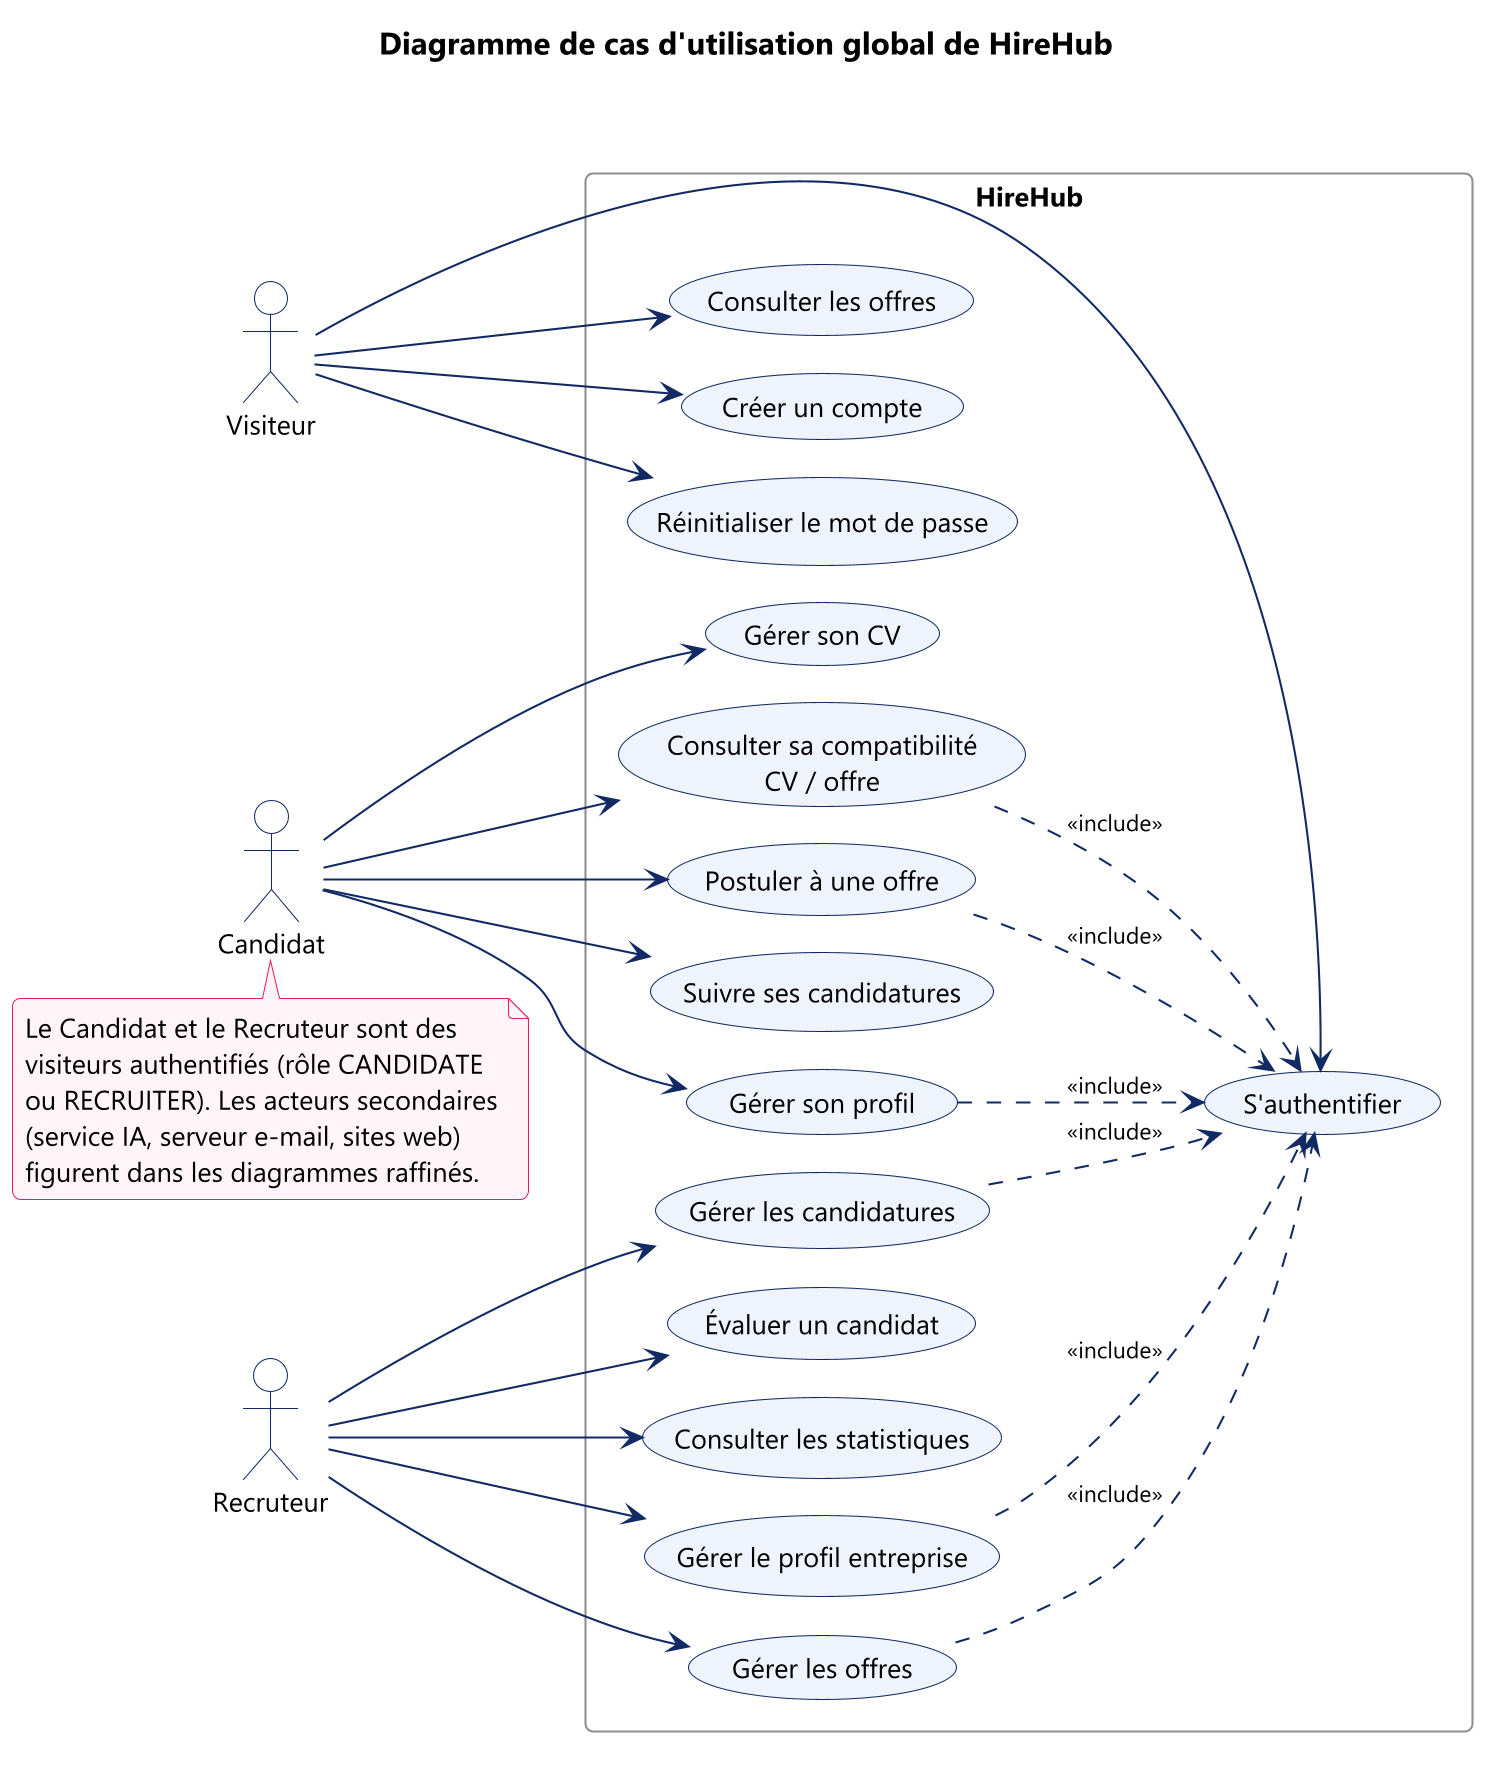
\includegraphics[width=0.8\textwidth,height=0.7\textheight,keepaspectratio]{cas-utilisation-global.png}
\caption{Diagramme de cas d'utilisation global}
\label{fig:uc-global}
\end{figure}

% ------------------------------------------------------------
\subsection{Analyse du cas d'utilisation « Gérer les offres »}

\subsubsection{Raffinement du cas d'utilisation « Gérer les offres »}
La figure \ref{fig:raf-offres} illustre en détail le cas d'utilisation « Gérer les offres » ainsi que ses sous-cas d'utilisation.

\begin{figure}[H]\centering
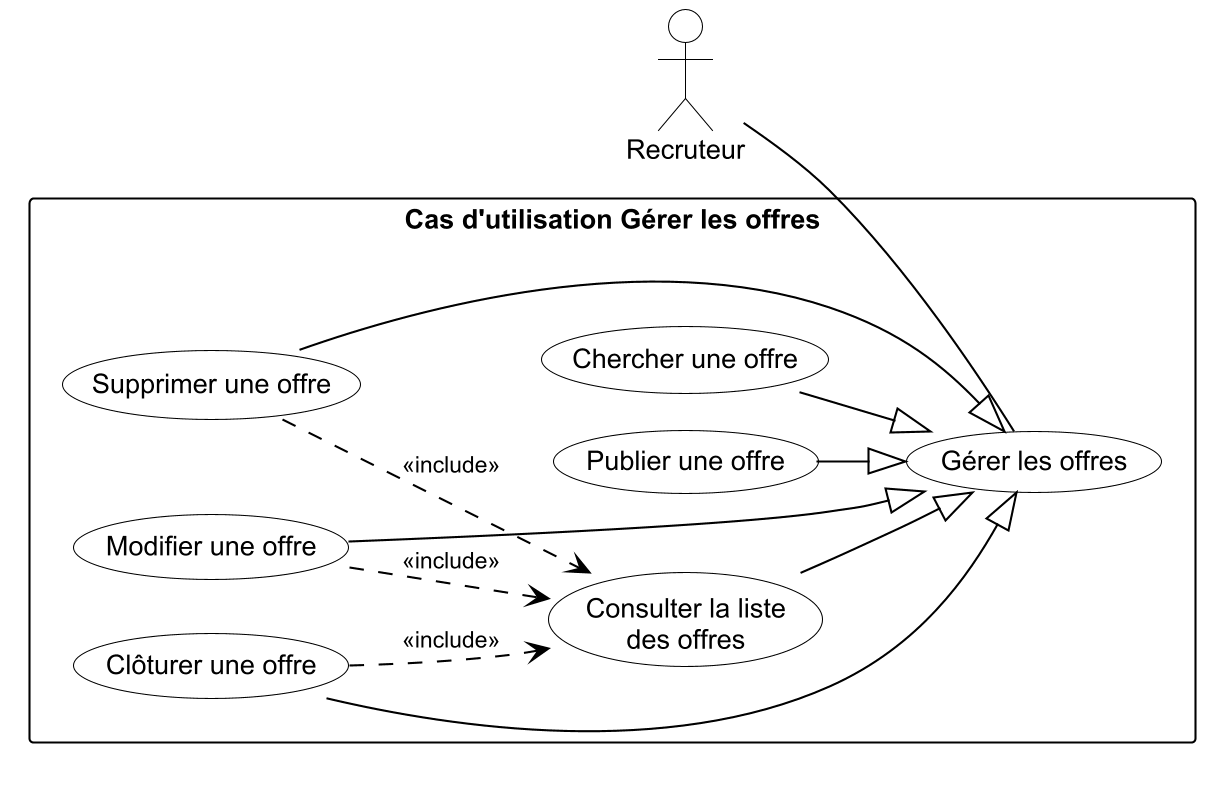
\includegraphics[width=0.85\textwidth,height=0.45\textheight,keepaspectratio]{raffinement-gerer-offres.png}
\caption{Raffinement du cas d'utilisation « Gérer les offres »}
\label{fig:raf-offres}
\end{figure}

\subsubsection{Description textuelle du cas d'utilisation « Publier une offre »}
Le tableau \ref{tab:desc-publier} présente la description textuelle du cas d'utilisation « Publier une offre ».

\begin{table}[H]
\centering\small
\begin{tabularx}{\textwidth}{|p{3.6cm}|L|}
\hline
\thead{Cas d'utilisation} & Publier une offre \\ \hline
\thead{Acteur principal} & Recruteur \\ \hline
\thead{Pré-conditions} & Le recruteur est authentifié. \\ \hline
\thead{Post-conditions} & L'offre est enregistrée avec le statut « ouverte » et visible par les candidats. \\ \hline
\thead{Scénario nominal} & 1. Le recruteur clique sur « New job offer ».\newline
2. Le système affiche le formulaire de l'offre.\newline
3. Le recruteur saisit le titre, la description, le lieu, le type de contrat et la date limite, puis clique sur « Publish ».\newline
4. Le système vérifie la validité des données, enregistre l'offre et affiche un message de succès. \\ \hline
\thead{Enchaînements alternatifs} & A1 : un champ obligatoire est vide ou invalide.\newline
A1.1 : le système affiche un message d'erreur sous le champ concerné.\newline
A1.2 : retour à l'étape 3 du scénario nominal. \\ \hline
\end{tabularx}
\caption{Description du cas d'utilisation « Publier une offre »}
\label{tab:desc-publier}
\end{table}

\subsubsection{Diagramme de séquence système du cas d'utilisation « Publier une offre »}
La figure \ref{fig:dss-publier} décrit les interactions entre le recruteur et le système.

\begin{figure}[H]\centering
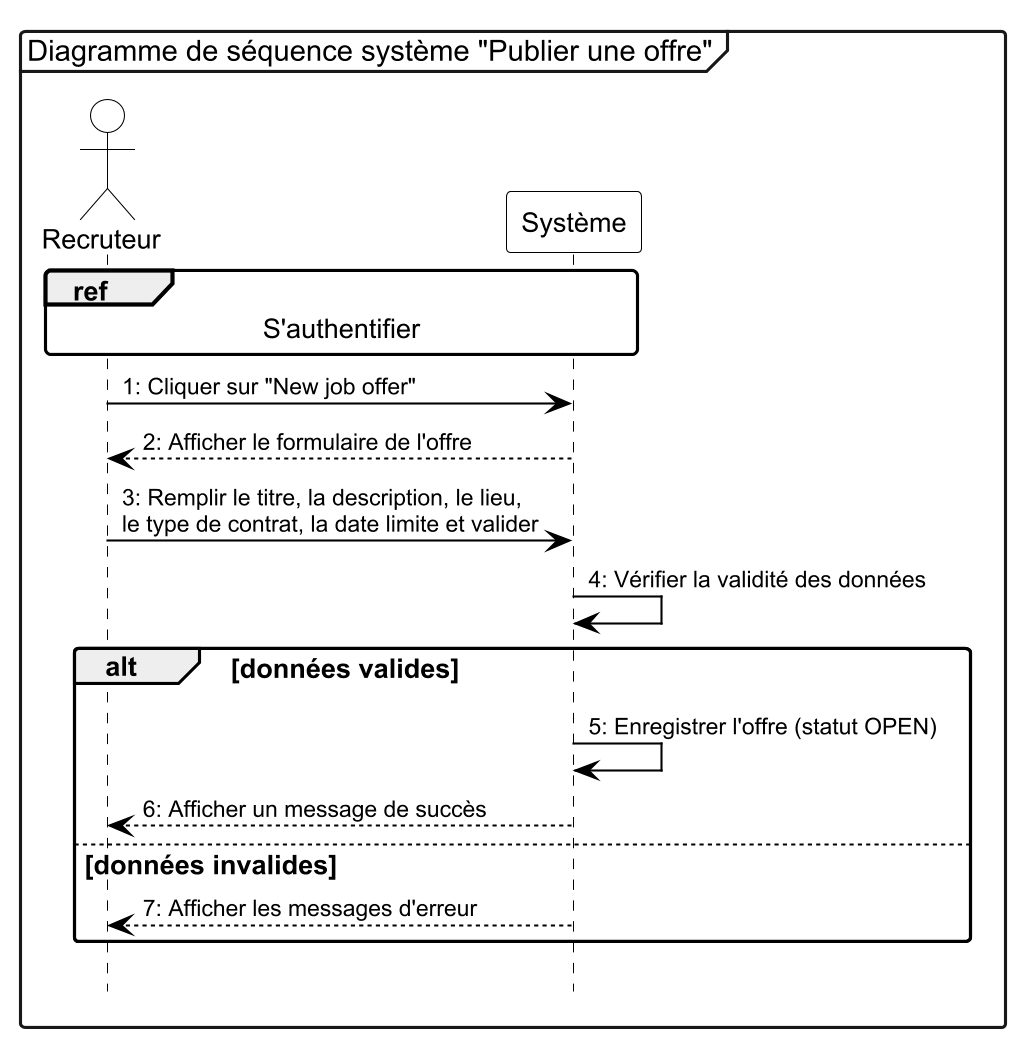
\includegraphics[width=0.8\textwidth,height=0.5\textheight,keepaspectratio]{dss-publier-offre.png}
\caption{Diagramme de séquence système « Publier une offre »}
\label{fig:dss-publier}
\end{figure}

% ------------------------------------------------------------
\subsection{Analyse du cas d'utilisation « Gérer les candidatures reçues »}

\subsubsection{Raffinement du cas d'utilisation « Gérer les candidatures reçues »}
La figure \ref{fig:raf-recues} offre une vue détaillée du cas d'utilisation « Gérer les candidatures reçues » et de ses sous-cas associés.

\begin{figure}[H]\centering
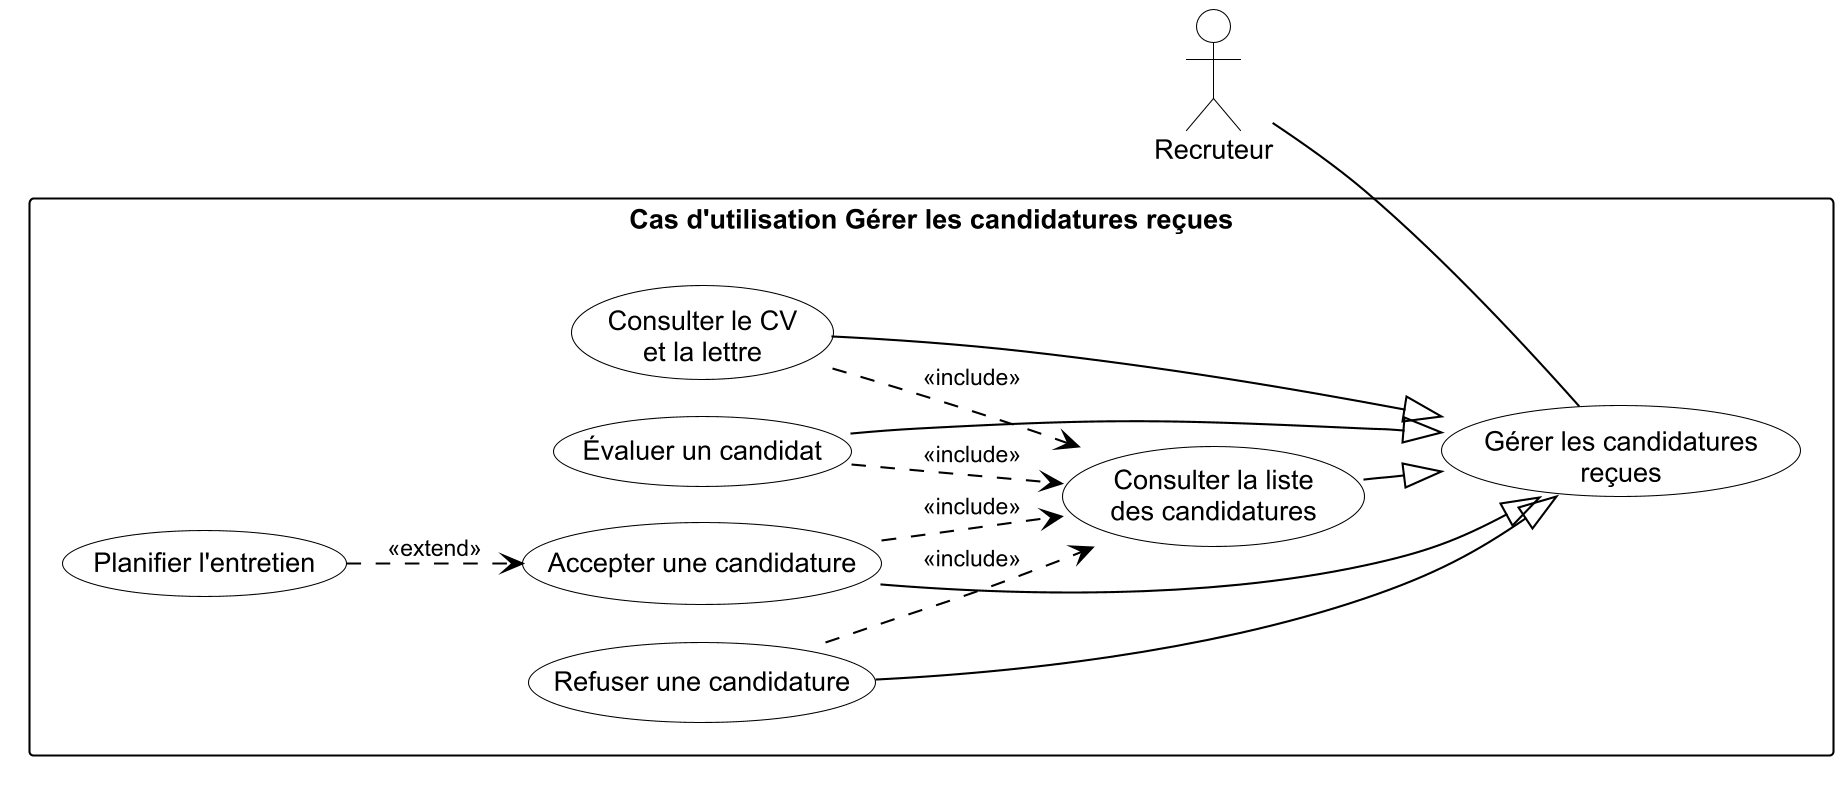
\includegraphics[width=0.85\textwidth,height=0.45\textheight,keepaspectratio]{raffinement-gerer-candidatures-recues.png}
\caption{Raffinement du cas d'utilisation « Gérer les candidatures reçues »}
\label{fig:raf-recues}
\end{figure}

\subsubsection{Description textuelle du cas d'utilisation « Accepter une candidature »}

\begin{table}[H]
\centering\small
\begin{tabularx}{\textwidth}{|p{3.6cm}|L|}
\hline
\thead{Cas d'utilisation} & Accepter une candidature \\ \hline
\thead{Acteur principal} & Recruteur \\ \hline
\thead{Pré-conditions} & Le recruteur est authentifié et propriétaire de l'offre ; la candidature est « en attente ». \\ \hline
\thead{Post-conditions} & La candidature est acceptée et le candidat reçoit une notification avec la date de l'entretien. \\ \hline
\thead{Scénario nominal} & 1. Le recruteur sélectionne une candidature et consulte le CV.\newline
2. Il clique sur « Accept… » et saisit la date et l'heure de l'entretien.\newline
3. Le système vérifie les droits du recruteur et l'état de la candidature.\newline
4. Le système enregistre la décision, notifie le candidat et affiche un message de succès. \\ \hline
\thead{Enchaînements alternatifs} & A1 : le recruteur n'est pas propriétaire de l'offre : accès refusé (HTTP 403).\newline
A2 : la candidature est déjà traitée : « Application has already been processed. »\newline
A3 : la date d'entretien manque : message d'erreur, retour à l'étape 2. \\ \hline
\end{tabularx}
\caption{Description du cas d'utilisation « Accepter une candidature »}
\end{table}

\subsubsection{Diagramme de séquence système du cas d'utilisation « Accepter une candidature »}

\begin{figure}[H]\centering
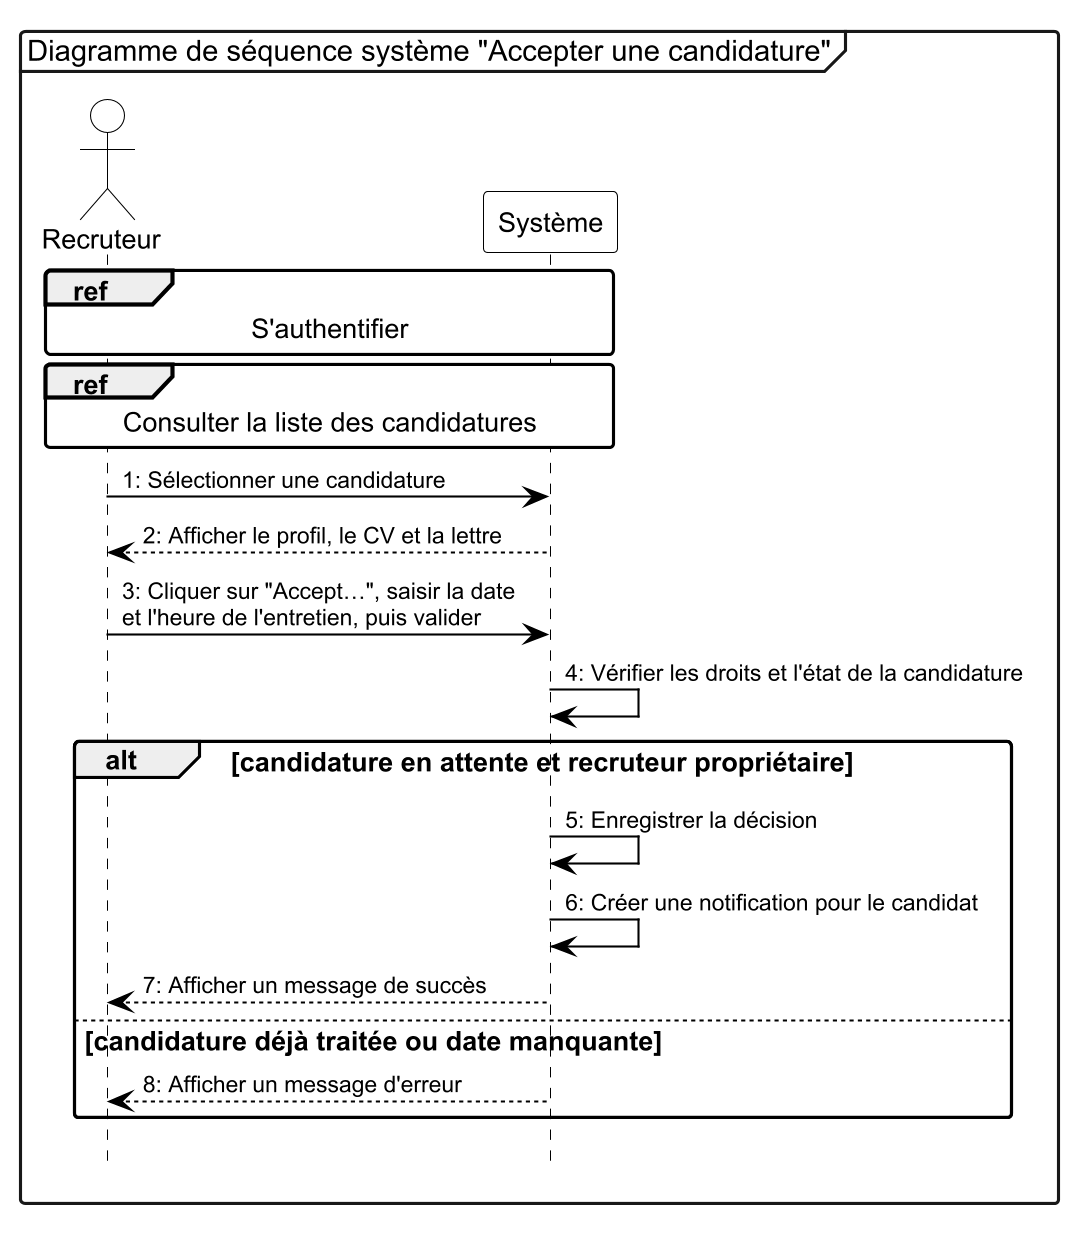
\includegraphics[width=0.8\textwidth,height=0.55\textheight,keepaspectratio]{dss-accepter-candidature.png}
\caption{Diagramme de séquence système « Accepter une candidature »}
\end{figure}

% ------------------------------------------------------------
\subsection{Analyse du cas d'utilisation « Gérer ses candidatures »}

\subsubsection{Raffinement du cas d'utilisation « Gérer ses candidatures »}

\begin{figure}[H]\centering
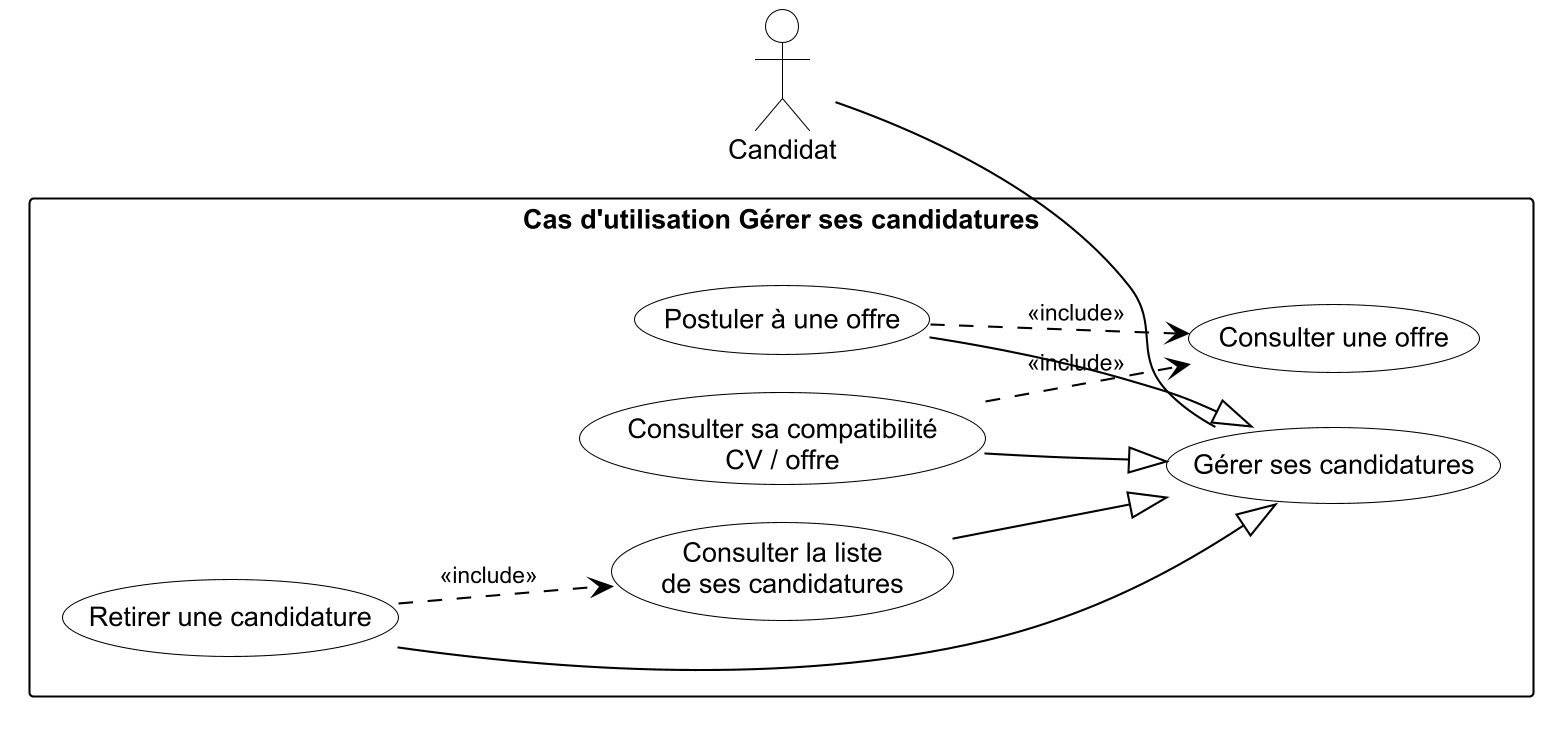
\includegraphics[width=0.85\textwidth,height=0.45\textheight,keepaspectratio]{raffinement-gerer-ses-candidatures.png}
\caption{Raffinement du cas d'utilisation « Gérer ses candidatures »}
\end{figure}

\subsubsection{Description textuelle du cas d'utilisation « Postuler à une offre »}

\begin{table}[H]
\centering\small
\begin{tabularx}{\textwidth}{|p{3.6cm}|L|}
\hline
\thead{Cas d'utilisation} & Postuler à une offre \\ \hline
\thead{Acteur principal} & Candidat \\ \hline
\thead{Pré-conditions} & Le candidat est authentifié ; l'offre est ouverte. \\ \hline
\thead{Post-conditions} & Une candidature « en attente » est créée. \\ \hline
\thead{Scénario nominal} & 1. Le candidat consulte une offre et clique sur « Apply Now ».\newline
2. Le système affiche le formulaire de candidature.\newline
3. Le candidat choisit son CV (PDF), rédige une lettre de motivation facultative et clique sur « Send application ».\newline
4. Le système vérifie le fichier (vrai PDF, 10 Mo maximum), l'offre et l'absence de candidature existante.\newline
5. Le système enregistre la candidature et affiche un message de succès. \\ \hline
\thead{Enchaînements alternatifs} & A1 : offre clôturée ou date limite dépassée : message d'erreur.\newline
A2 : candidature déjà existante : « You have already applied for this job offer. »\newline
A3 : fichier invalide : message d'erreur, retour à l'étape 3. \\ \hline
\end{tabularx}
\caption{Description du cas d'utilisation « Postuler à une offre »}
\end{table}

\subsubsection{Diagramme de séquence système du cas d'utilisation « Postuler à une offre »}

\begin{figure}[H]\centering
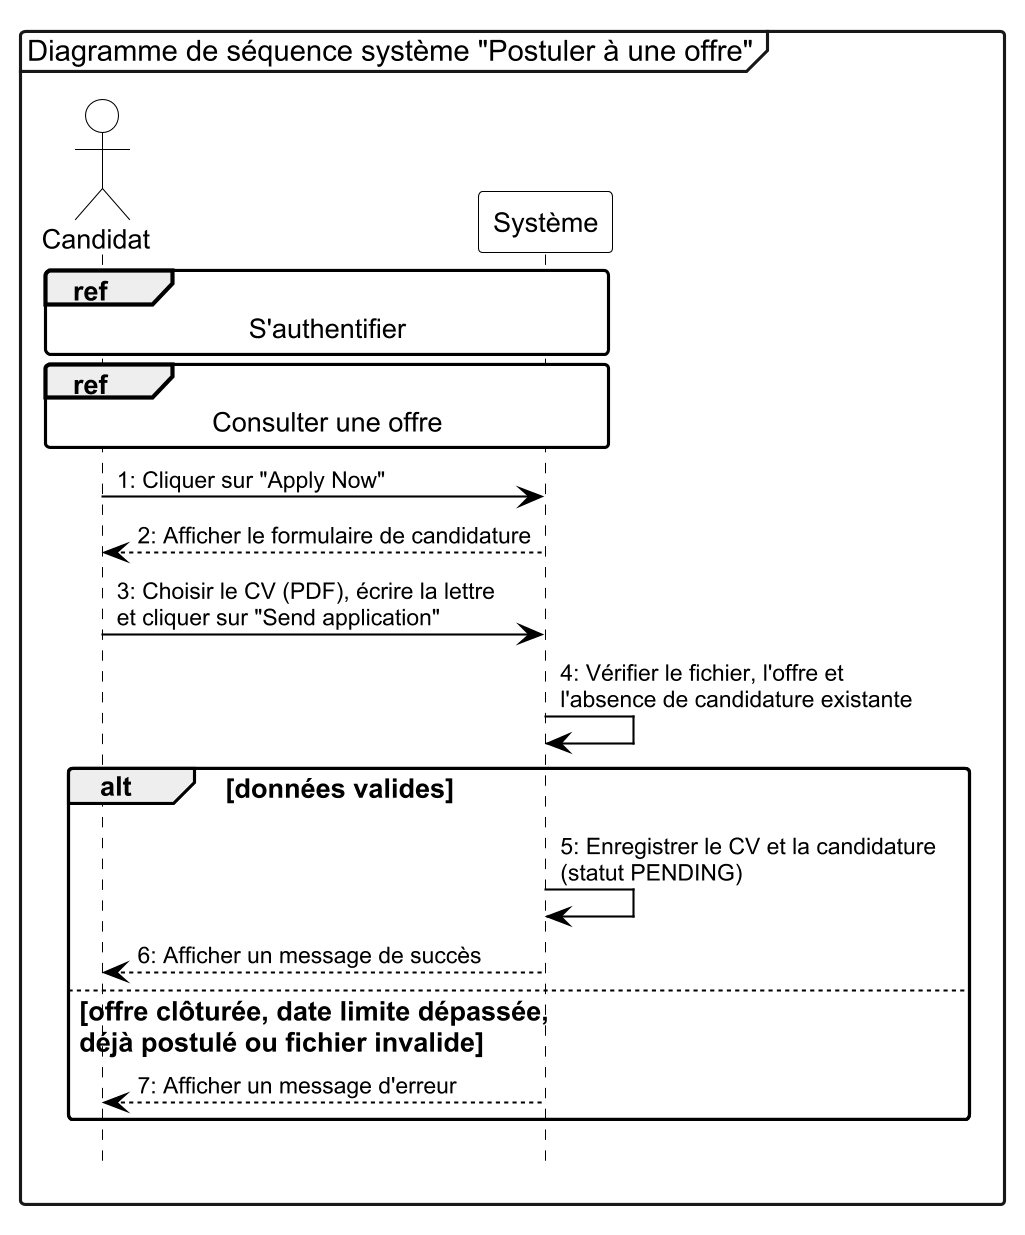
\includegraphics[width=0.8\textwidth,height=0.55\textheight,keepaspectratio]{dss-postuler-offre.png}
\caption{Diagramme de séquence système « Postuler à une offre »}
\end{figure}

% ------------------------------------------------------------
\subsection{Analyse du cas d'utilisation « Gérer le profil entreprise »}

\subsubsection{Raffinement du cas d'utilisation « Gérer le profil entreprise »}

\begin{figure}[H]\centering
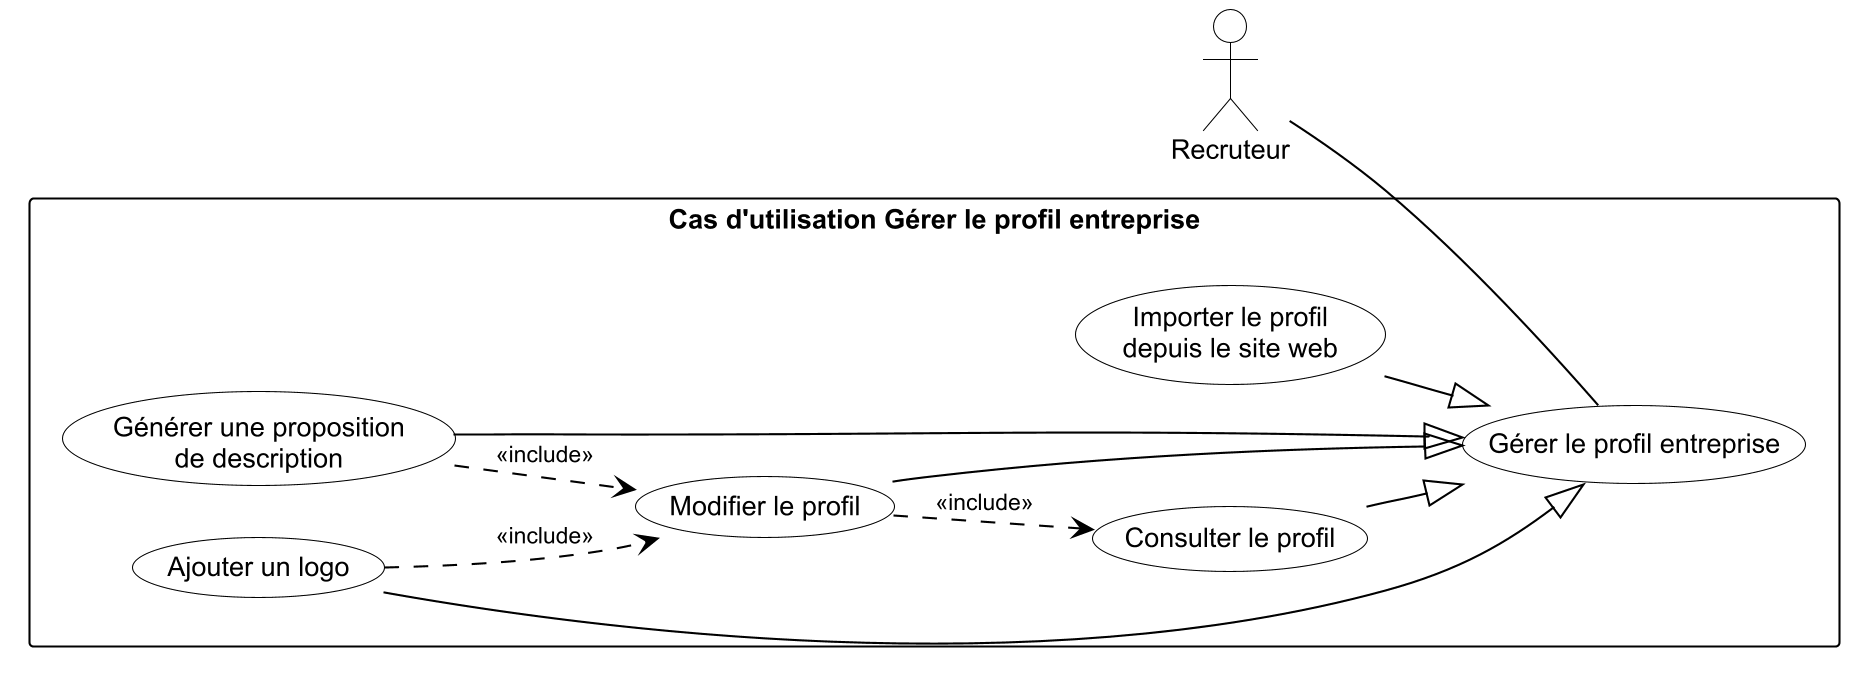
\includegraphics[width=0.85\textwidth,height=0.45\textheight,keepaspectratio]{raffinement-gerer-profil-entreprise.png}
\caption{Raffinement du cas d'utilisation « Gérer le profil entreprise »}
\end{figure}

\subsubsection{Description textuelle du cas d'utilisation « Importer le profil depuis le site web »}

\begin{table}[H]
\centering\small
\begin{tabularx}{\textwidth}{|p{3.6cm}|L|}
\hline
\thead{Cas d'utilisation} & Importer le profil depuis le site web \\ \hline
\thead{Acteur principal} & Recruteur \\ \hline
\thead{Acteur secondaire} & Site web de l'entreprise \\ \hline
\thead{Pré-conditions} & Le recruteur est authentifié et a renseigné l'adresse du site web. \\ \hline
\thead{Post-conditions} & Les champs vides du profil sont remplis et marqués « From your website ». \\ \hline
\thead{Scénario nominal} & 1. Le recruteur clique sur « Fill empty fields from this website ».\newline
2. Le système vérifie que l'adresse est publique.\newline
3. Le système affiche une bannière de progression et lit les pages publiques du site.\newline
4. Le système extrait les informations et remplit uniquement les champs vides.\newline
5. Le système affiche les champs remplis. \\ \hline
\thead{Enchaînements alternatifs} & A1 : adresse interne ou privée : l'import est refusé (protection SSRF).\newline
A2 : site inaccessible : message d'erreur et bouton « Try again ». \\ \hline
\end{tabularx}
\caption{Description du cas d'utilisation « Importer le profil depuis le site web »}
\end{table}

\subsubsection{Diagramme de séquence système du cas d'utilisation « Importer le profil depuis le site web »}

\begin{figure}[H]\centering
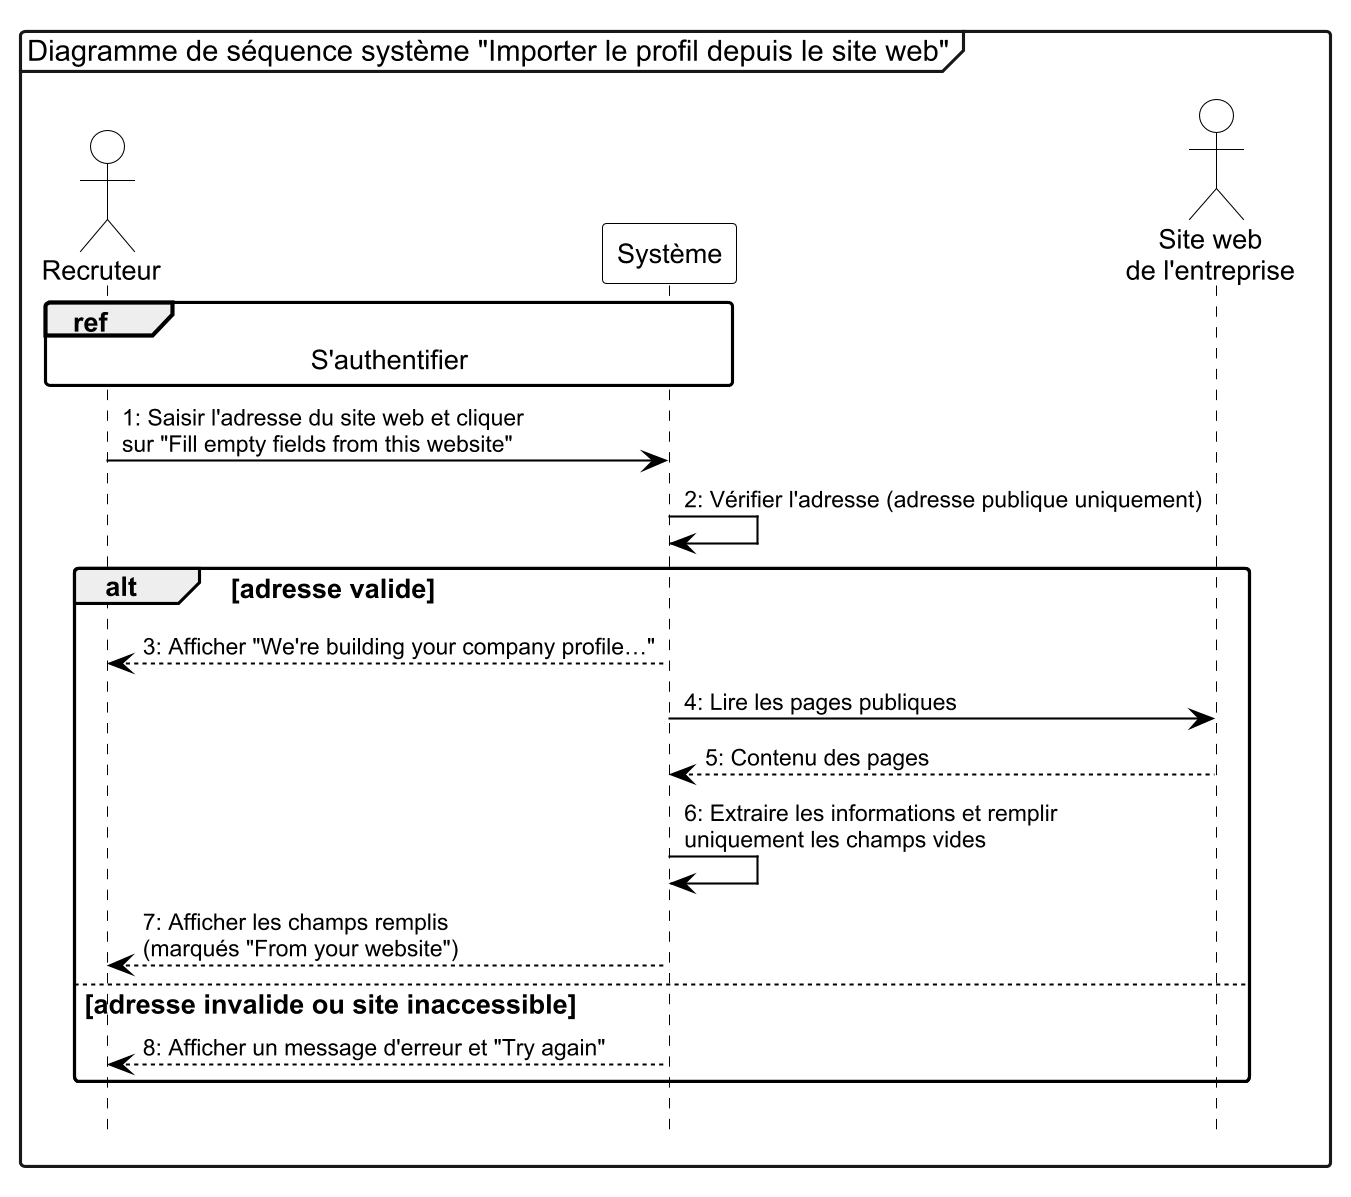
\includegraphics[width=0.85\textwidth,height=0.55\textheight,keepaspectratio]{dss-importer-profil.png}
\caption{Diagramme de séquence système « Importer le profil depuis le site web »}
\end{figure}

\section{Backlog du produit}
Le backlog du produit regroupe les fonctionnalités sous forme d'histoires utilisateur (user stories), classées par priorité (tableau \ref{tab:backlog}).

\begin{longtable}{|p{0.6cm}|p{3cm}|p{8.6cm}|p{1.6cm}|}
\hline
\rowcolor{headgray}\thead{ID} & \thead{Fonctionnalité} & \thead{User story} & \thead{Priorité} \\ \hline
\endfirsthead
\hline
\rowcolor{headgray}\thead{ID} & \thead{Fonctionnalité} & \thead{User story} & \thead{Priorité} \\ \hline
\endhead
01 & Authentification & En tant que visiteur, je veux créer un compte et être connecté directement. & Élevée \\ \cline{3-4}
 & & En tant qu'utilisateur, je veux réinitialiser mon mot de passe par e-mail. & Élevée \\ \hline
02 & Gestion des offres & En tant que recruteur, je veux publier, modifier et supprimer une offre. & Élevée \\ \cline{3-4}
 & & En tant que recruteur, je veux clôturer une offre sans perdre ses candidats. & Moyenne \\ \hline
03 & Recherche d'offres & En tant que candidat, je veux filtrer les offres par mot-clé, lieu et contrat. & Élevée \\ \hline
04 & CV & En tant que candidat, je veux déposer mon CV et le prévisualiser. & Élevée \\ \hline
05 & Compatibilité & En tant que candidat, je veux connaître mon score de compatibilité avec une offre et savoir ce qui me manque. & Élevée \\ \hline
06 & Candidatures & En tant que candidat, je veux postuler et suivre l'état de mes candidatures. & Élevée \\ \cline{3-4}
 & & En tant que recruteur, je veux accepter (avec une date d'entretien) ou refuser une candidature. & Élevée \\ \hline
07 & Évaluation & En tant que recruteur, je veux évaluer un candidat selon des critères et obtenir une note sur 20. & Moyenne \\ \hline
08 & Profil entreprise & En tant que recruteur, je veux importer le profil de mon entreprise depuis son site web. & Moyenne \\ \hline
09 & Statistiques & En tant que recruteur, je veux consulter des statistiques sur mes offres et candidatures. & Moyenne \\ \hline
10 & Profils & En tant qu'utilisateur, je veux compléter mon profil et obtenir une proposition de texte basée sur mes données. & Faible \\ \hline
11 & E-mails & En tant qu'utilisateur, je veux recevoir un e-mail de bienvenue. & Faible \\ \hline
\caption{Backlog du produit}\label{tab:backlog}\\
\end{longtable}
% TODO Marwa: si vous voulez ajouter un planning (itérations avec dates), mettez vos dates réelles.

\section*{Conclusion}
\addcontentsline{toc}{section}{Conclusion}
Ce chapitre a permis d'identifier les acteurs, de détailler les besoins fonctionnels et non fonctionnels et de les représenter par des cas d'utilisation. Le chapitre suivant présente la conception de la solution.

% ============================================================
%  CHAPITRE 3
% ============================================================
\chapter{Conception}
\plan

\section*{Introduction}
\addcontentsline{toc}{section}{Introduction}
Ce chapitre présente la conception de HireHub. Nous décrivons d'abord l'architecture physique et logique, puis la conception détaillée à travers le diagramme de classes et les diagrammes de séquence objet.

\section{Architecture générale}

\subsection{Architecture physique}
HireHub suit une architecture \textbf{multi-tiers} composée de plusieurs services, chacun déployé dans son propre conteneur Docker (figure \ref{fig:arch-physique}) :
\begin{itemize}
  \item \textbf{frontend} : un serveur nginx sert l'application React et redirige les appels \texttt{/api} vers le backend ; c'est le seul service ouvert au réseau ;
  \item \textbf{backend} : l'API REST Spring Boot (Java 17) ;
  \item \textbf{ai-service} : le service d'analyse FastAPI (Python), accessible uniquement par le backend, avec une clé interne ;
  \item \textbf{mysql} : la base de données MySQL 8 ;
  \item \textbf{mailpit} : une boîte e-mail locale pour le développement (Gmail SMTP pour les vrais e-mails).
\end{itemize}

\begin{figure}[H]\centering
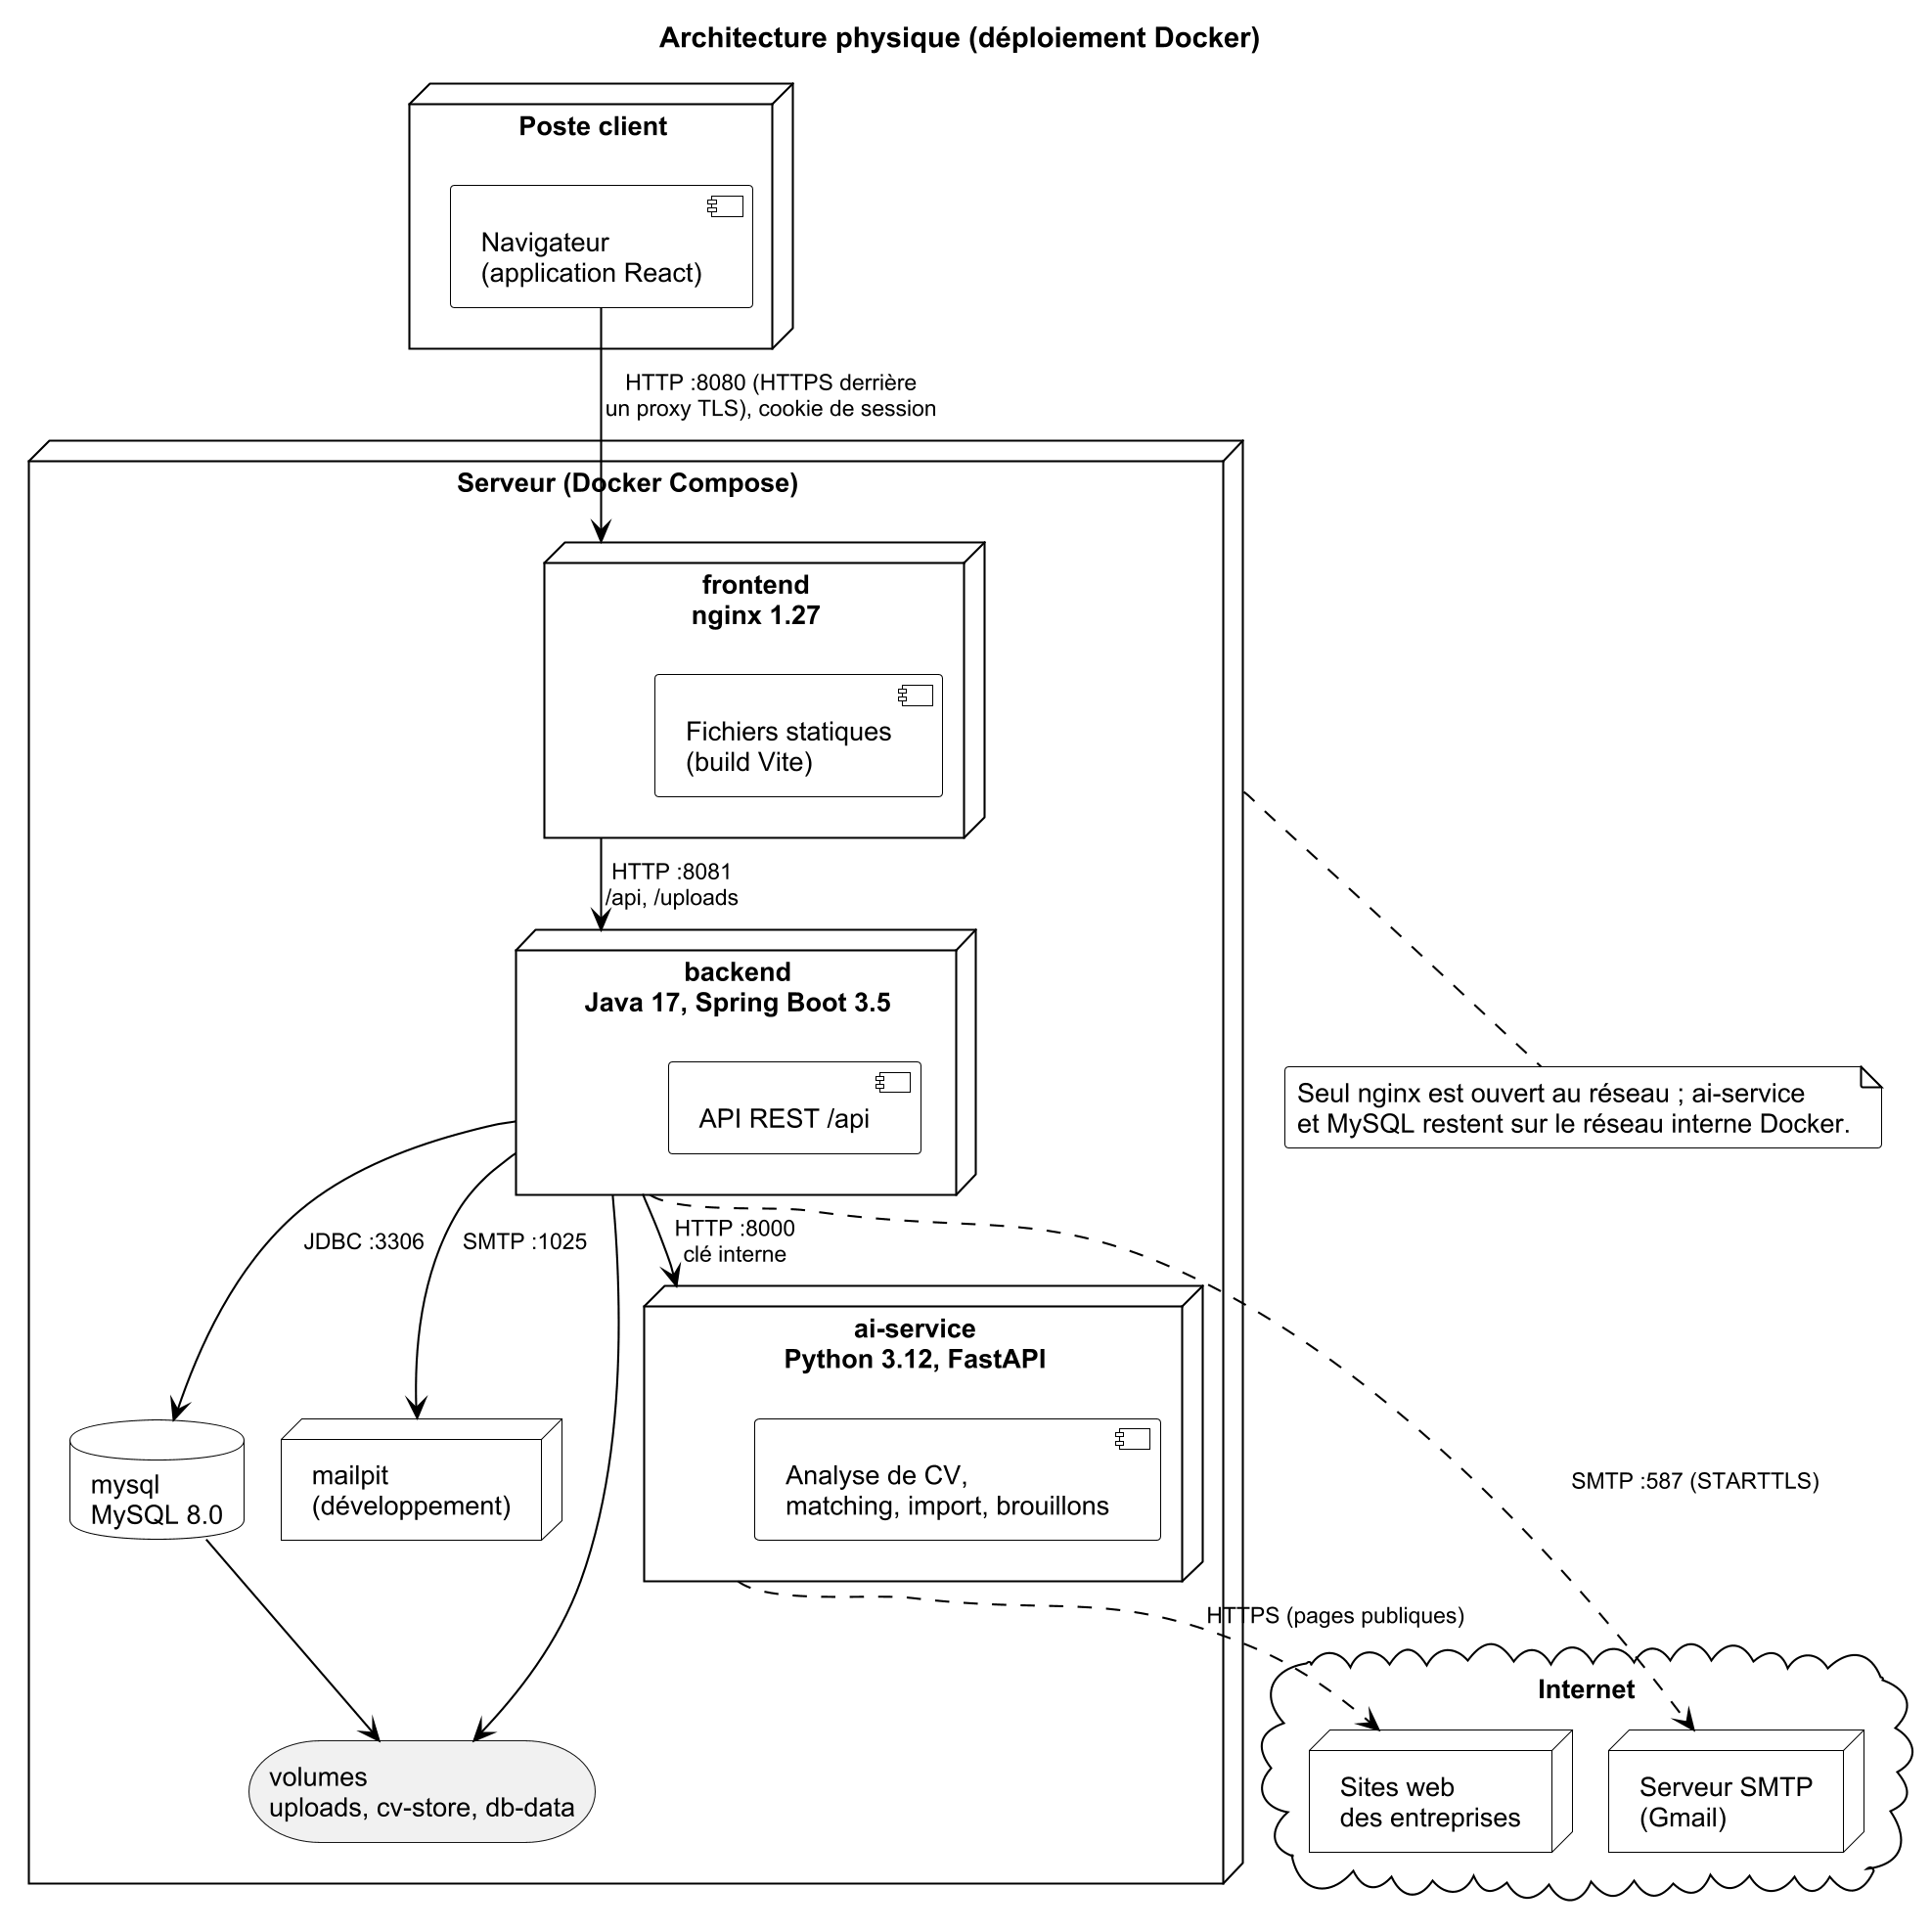
\includegraphics[width=0.85\textwidth,height=0.7\textheight,keepaspectratio]{architecture-physique.png}
\caption{Architecture physique (déploiement Docker)}
\label{fig:arch-physique}
\end{figure}

\subsection{Architecture logique}
Chaque service est organisé en couches (figure \ref{fig:arch-logique}). Côté backend, nous retrouvons le patron \textbf{MVC} adapté à une API REST : les contrôleurs reçoivent les requêtes, les services portent les règles métier, les repositories accèdent aux données, et les DTO séparent le modèle de données de l'API exposée.

\begin{table}[H]
\centering
\begin{tabularx}{\textwidth}{|p{3.4cm}|L|}
\hline
\rowcolor{headgray}\thead{Couche} & \thead{Rôle} \\ \hline
Filtres de sécurité & Identifiant de requête, lecture de la session (JWT), vérification CSRF, limitation de débit. \\ \hline
Controller & Expose les endpoints REST et délègue le traitement aux services. \\ \hline
Service & Contient la logique métier : règles de gestion et vérifications d'autorisation. \\ \hline
Repository & Accès à la base de données via Spring Data JPA. \\ \hline
DTO & Données échangées avec le frontend, indépendantes des entités. \\ \hline
Entity & Tables de la base, dont le schéma est versionné par Flyway. \\ \hline
Exception & Gestion centralisée des erreurs (\texttt{GlobalExceptionHandler}) avec un format unique. \\ \hline
\end{tabularx}
\caption{Couches du backend}
\end{table}

\begin{figure}[H]\centering
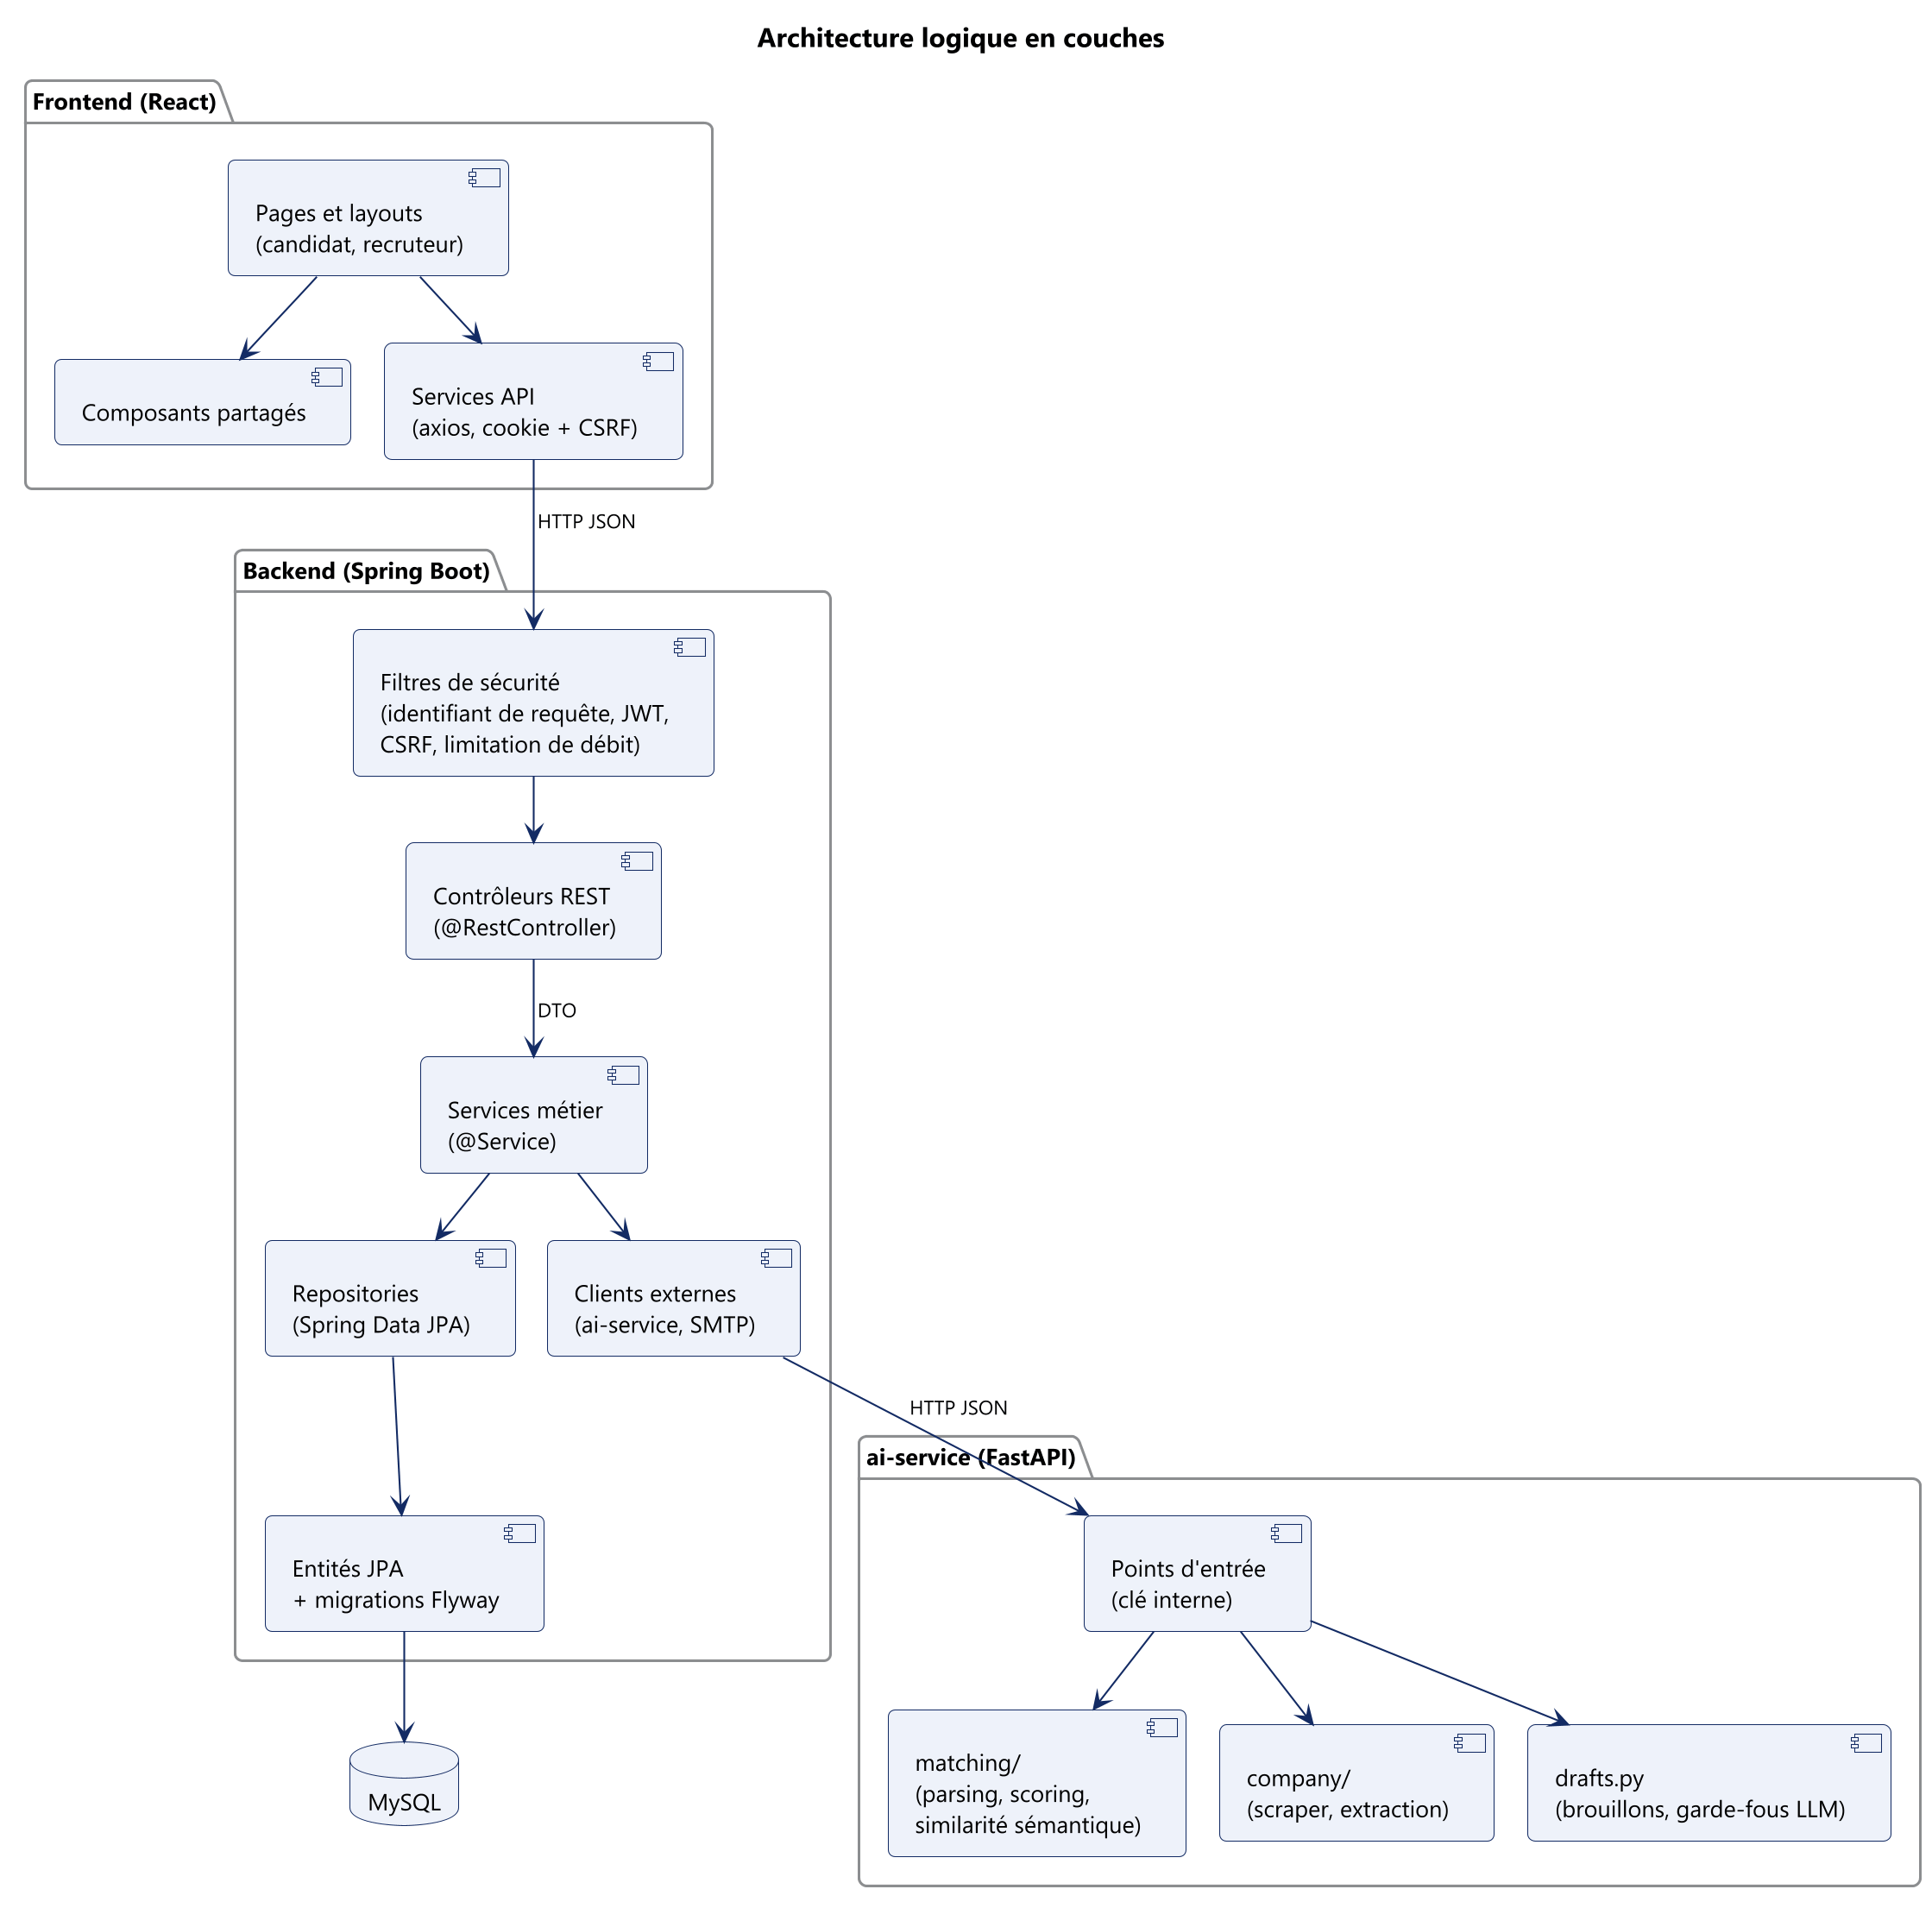
\includegraphics[width=0.85\textwidth,height=0.62\textheight,keepaspectratio]{architecture-logique.png}
\caption{Architecture logique en couches}
\label{fig:arch-logique}
\end{figure}

\section{Conception détaillée}

\subsection{Diagramme de classes}
Dans cette section, nous examinons l'aspect statique de notre application à travers le diagramme de classes. La figure \ref{fig:classes} présente les entités du système, leurs attributs, les opérations offertes par les services associés et les relations entre elles.

\begin{figure}[H]\centering
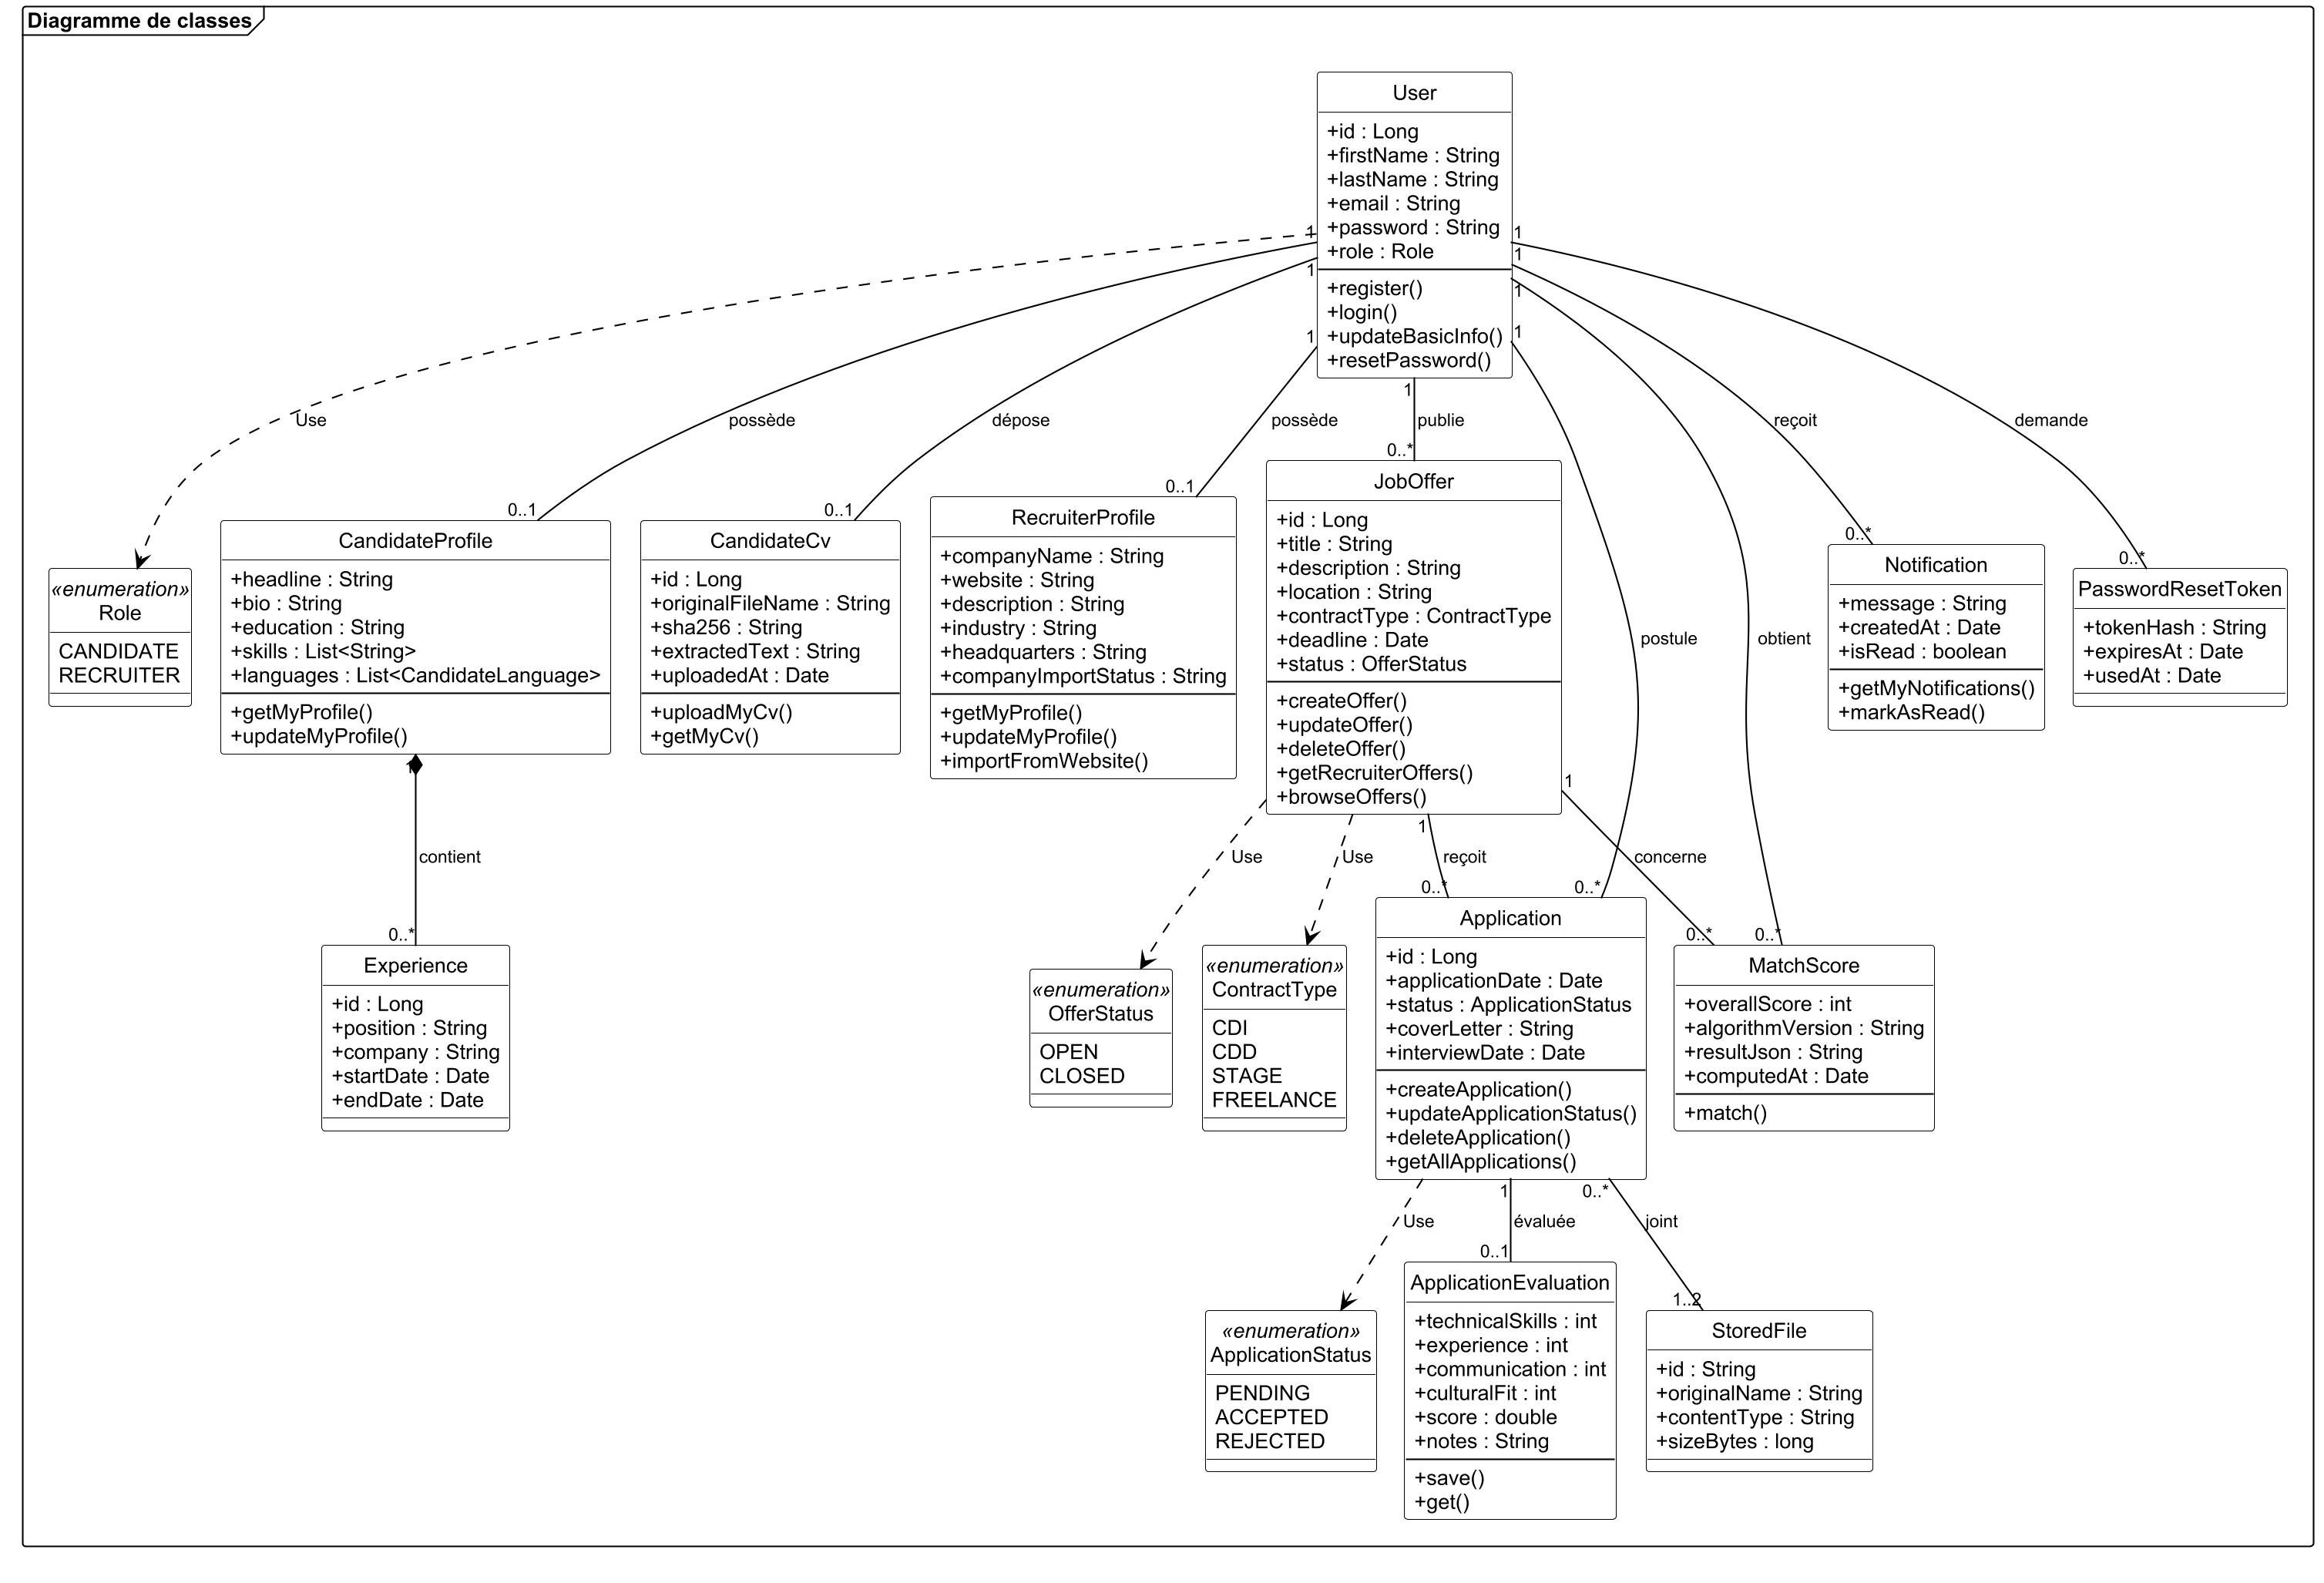
\includegraphics[width=\textwidth,height=0.75\textheight,keepaspectratio]{classes.png}
\caption{Diagramme de classes}
\label{fig:classes}
\end{figure}

\subsection{Diagrammes de séquence objet}
Au cours de cette section, nous examinons l'aspect dynamique de notre application. Ces diagrammes détaillent les échanges entre l'interface (\emph{View}), les contrôleurs, les entités et la base de données pour réaliser les principaux scénarios.

\subsubsection{Diagramme de séquence objet relatif au scénario « Publier une offre »}
\begin{figure}[H]\centering
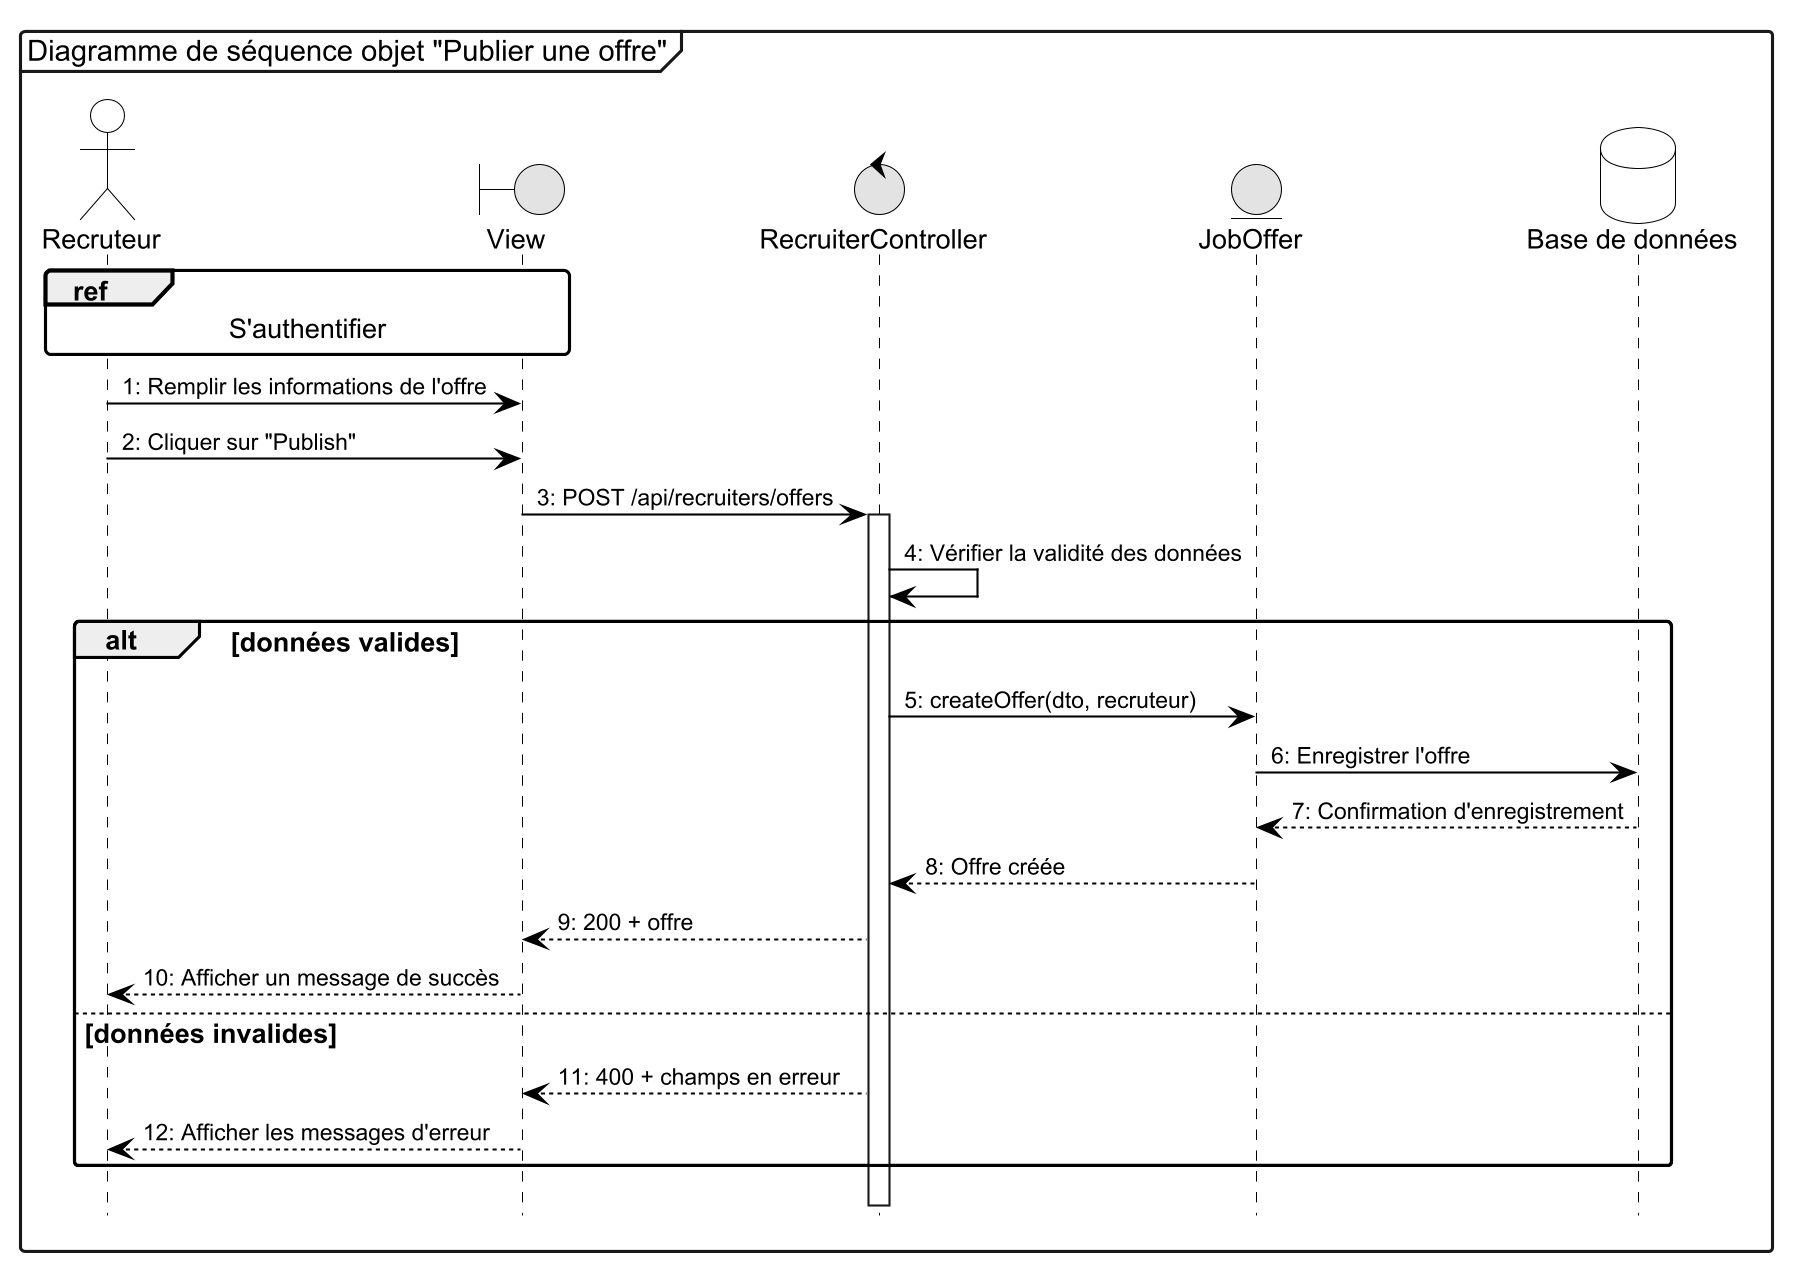
\includegraphics[width=\textwidth,height=0.6\textheight,keepaspectratio]{dso-publier-offre.png}
\caption{Diagramme de séquence objet relatif au scénario « Publier une offre »}
\end{figure}

\subsubsection{Diagramme de séquence objet relatif au scénario « Accepter une candidature »}
\begin{figure}[H]\centering
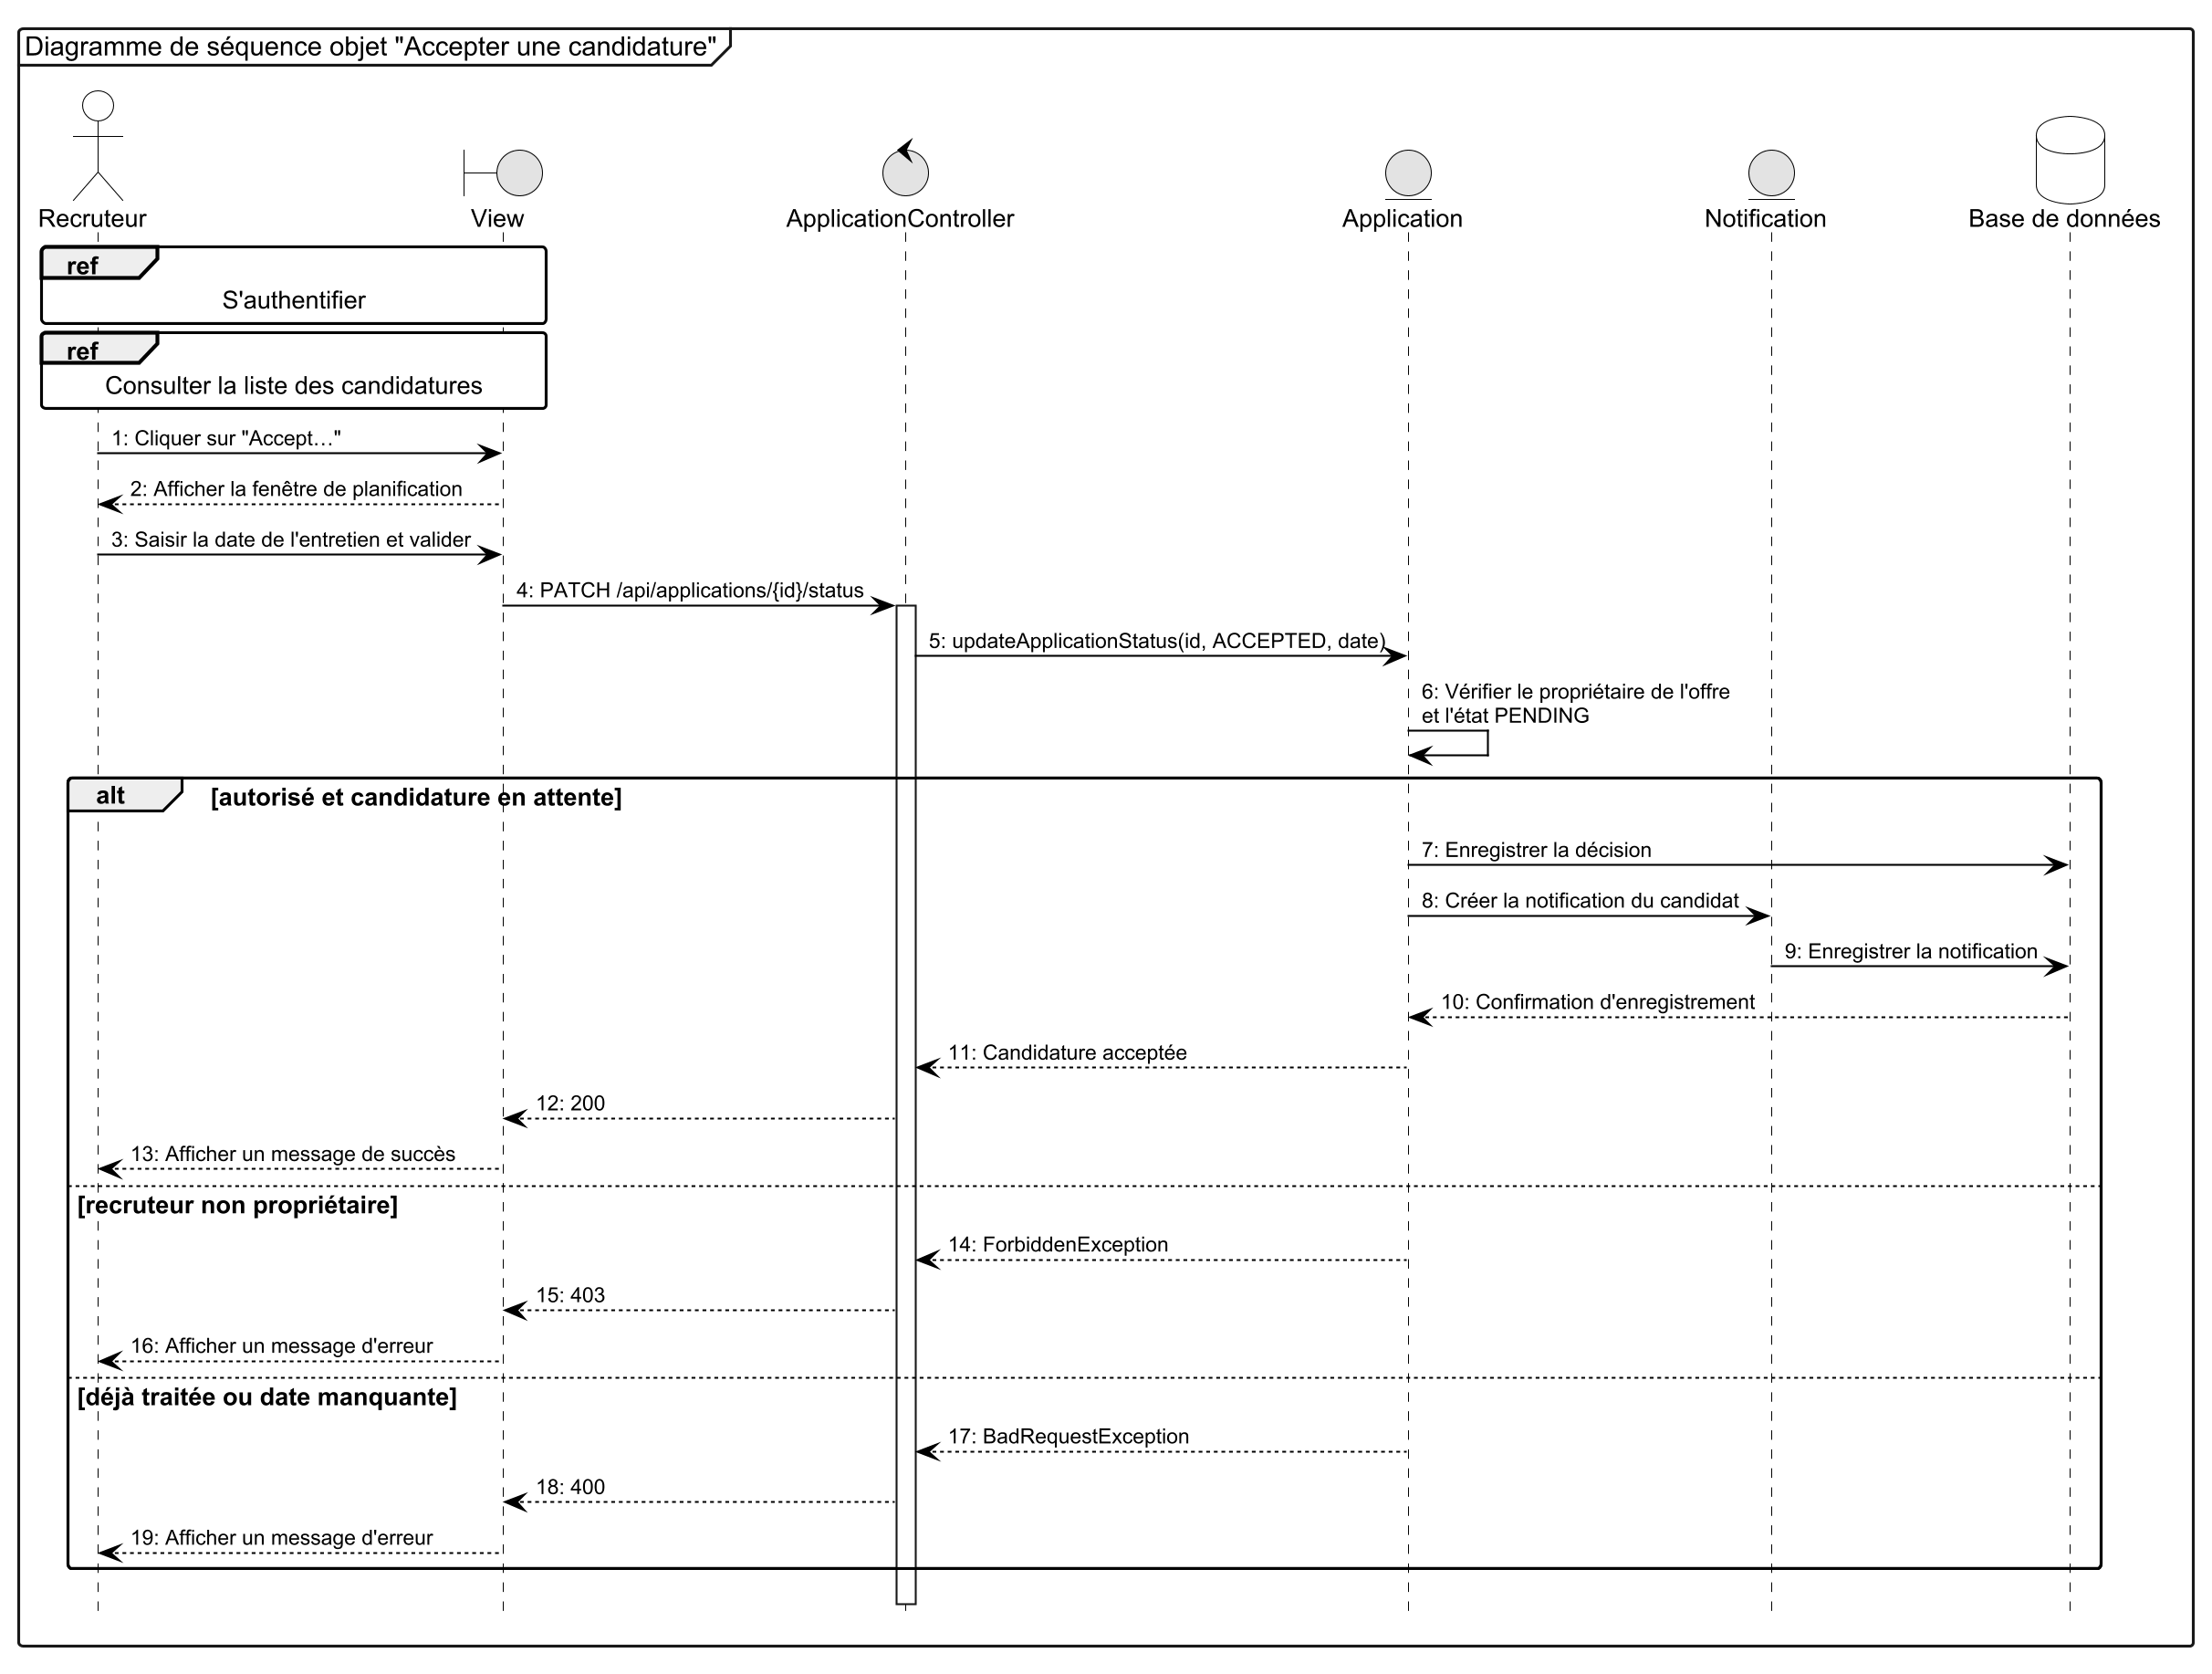
\includegraphics[width=\textwidth,height=0.7\textheight,keepaspectratio]{dso-accepter-candidature.png}
\caption{Diagramme de séquence objet relatif au scénario « Accepter une candidature »}
\end{figure}

\subsubsection{Diagramme de séquence objet relatif au scénario « Postuler à une offre »}
Dans ce scénario, le CV est d'abord enregistré dans un espace privé, puis la candidature est créée en référençant ce fichier.

\begin{figure}[H]\centering
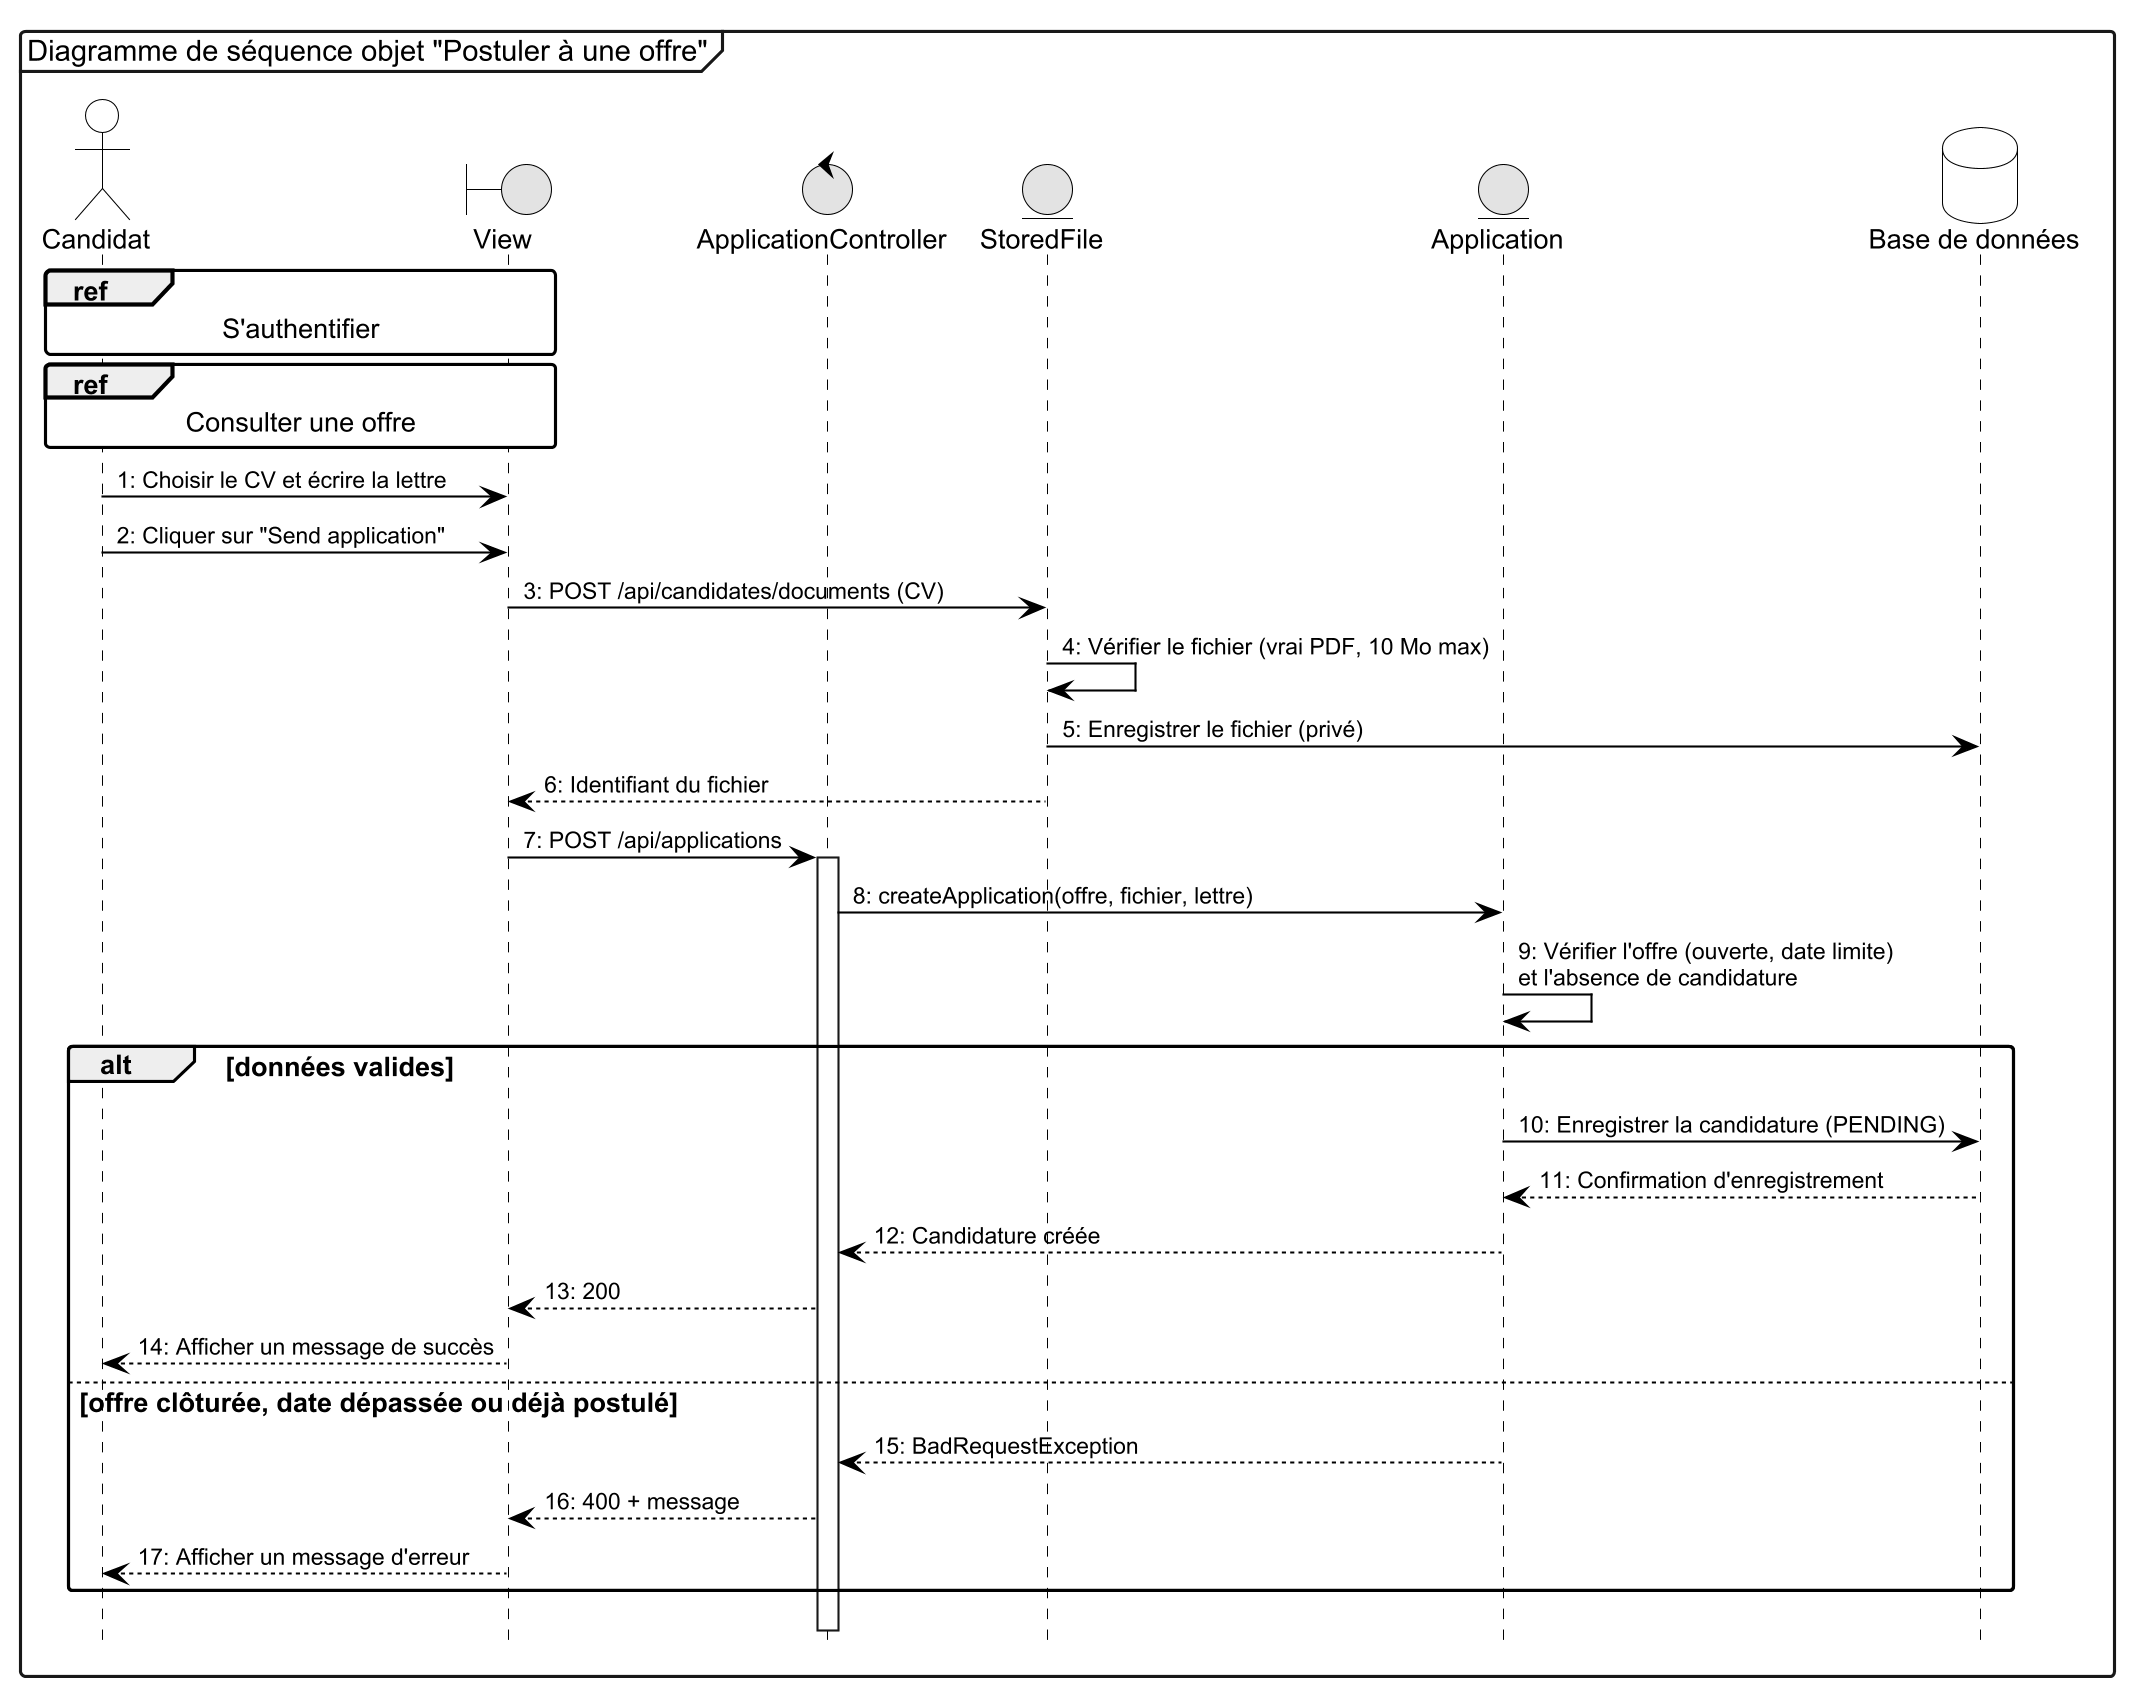
\includegraphics[width=\textwidth,height=0.7\textheight,keepaspectratio]{dso-postuler-offre.png}
\caption{Diagramme de séquence objet relatif au scénario « Postuler à une offre »}
\end{figure}

\subsubsection{Diagramme de séquence objet relatif au scénario « Consulter sa compatibilité CV / offre »}
Le résultat est mis en cache : il n'est recalculé que si le CV, le texte de l'offre ou la version de l'algorithme change. Si le service IA est indisponible, aucun score n'est affiché.

\begin{figure}[H]\centering
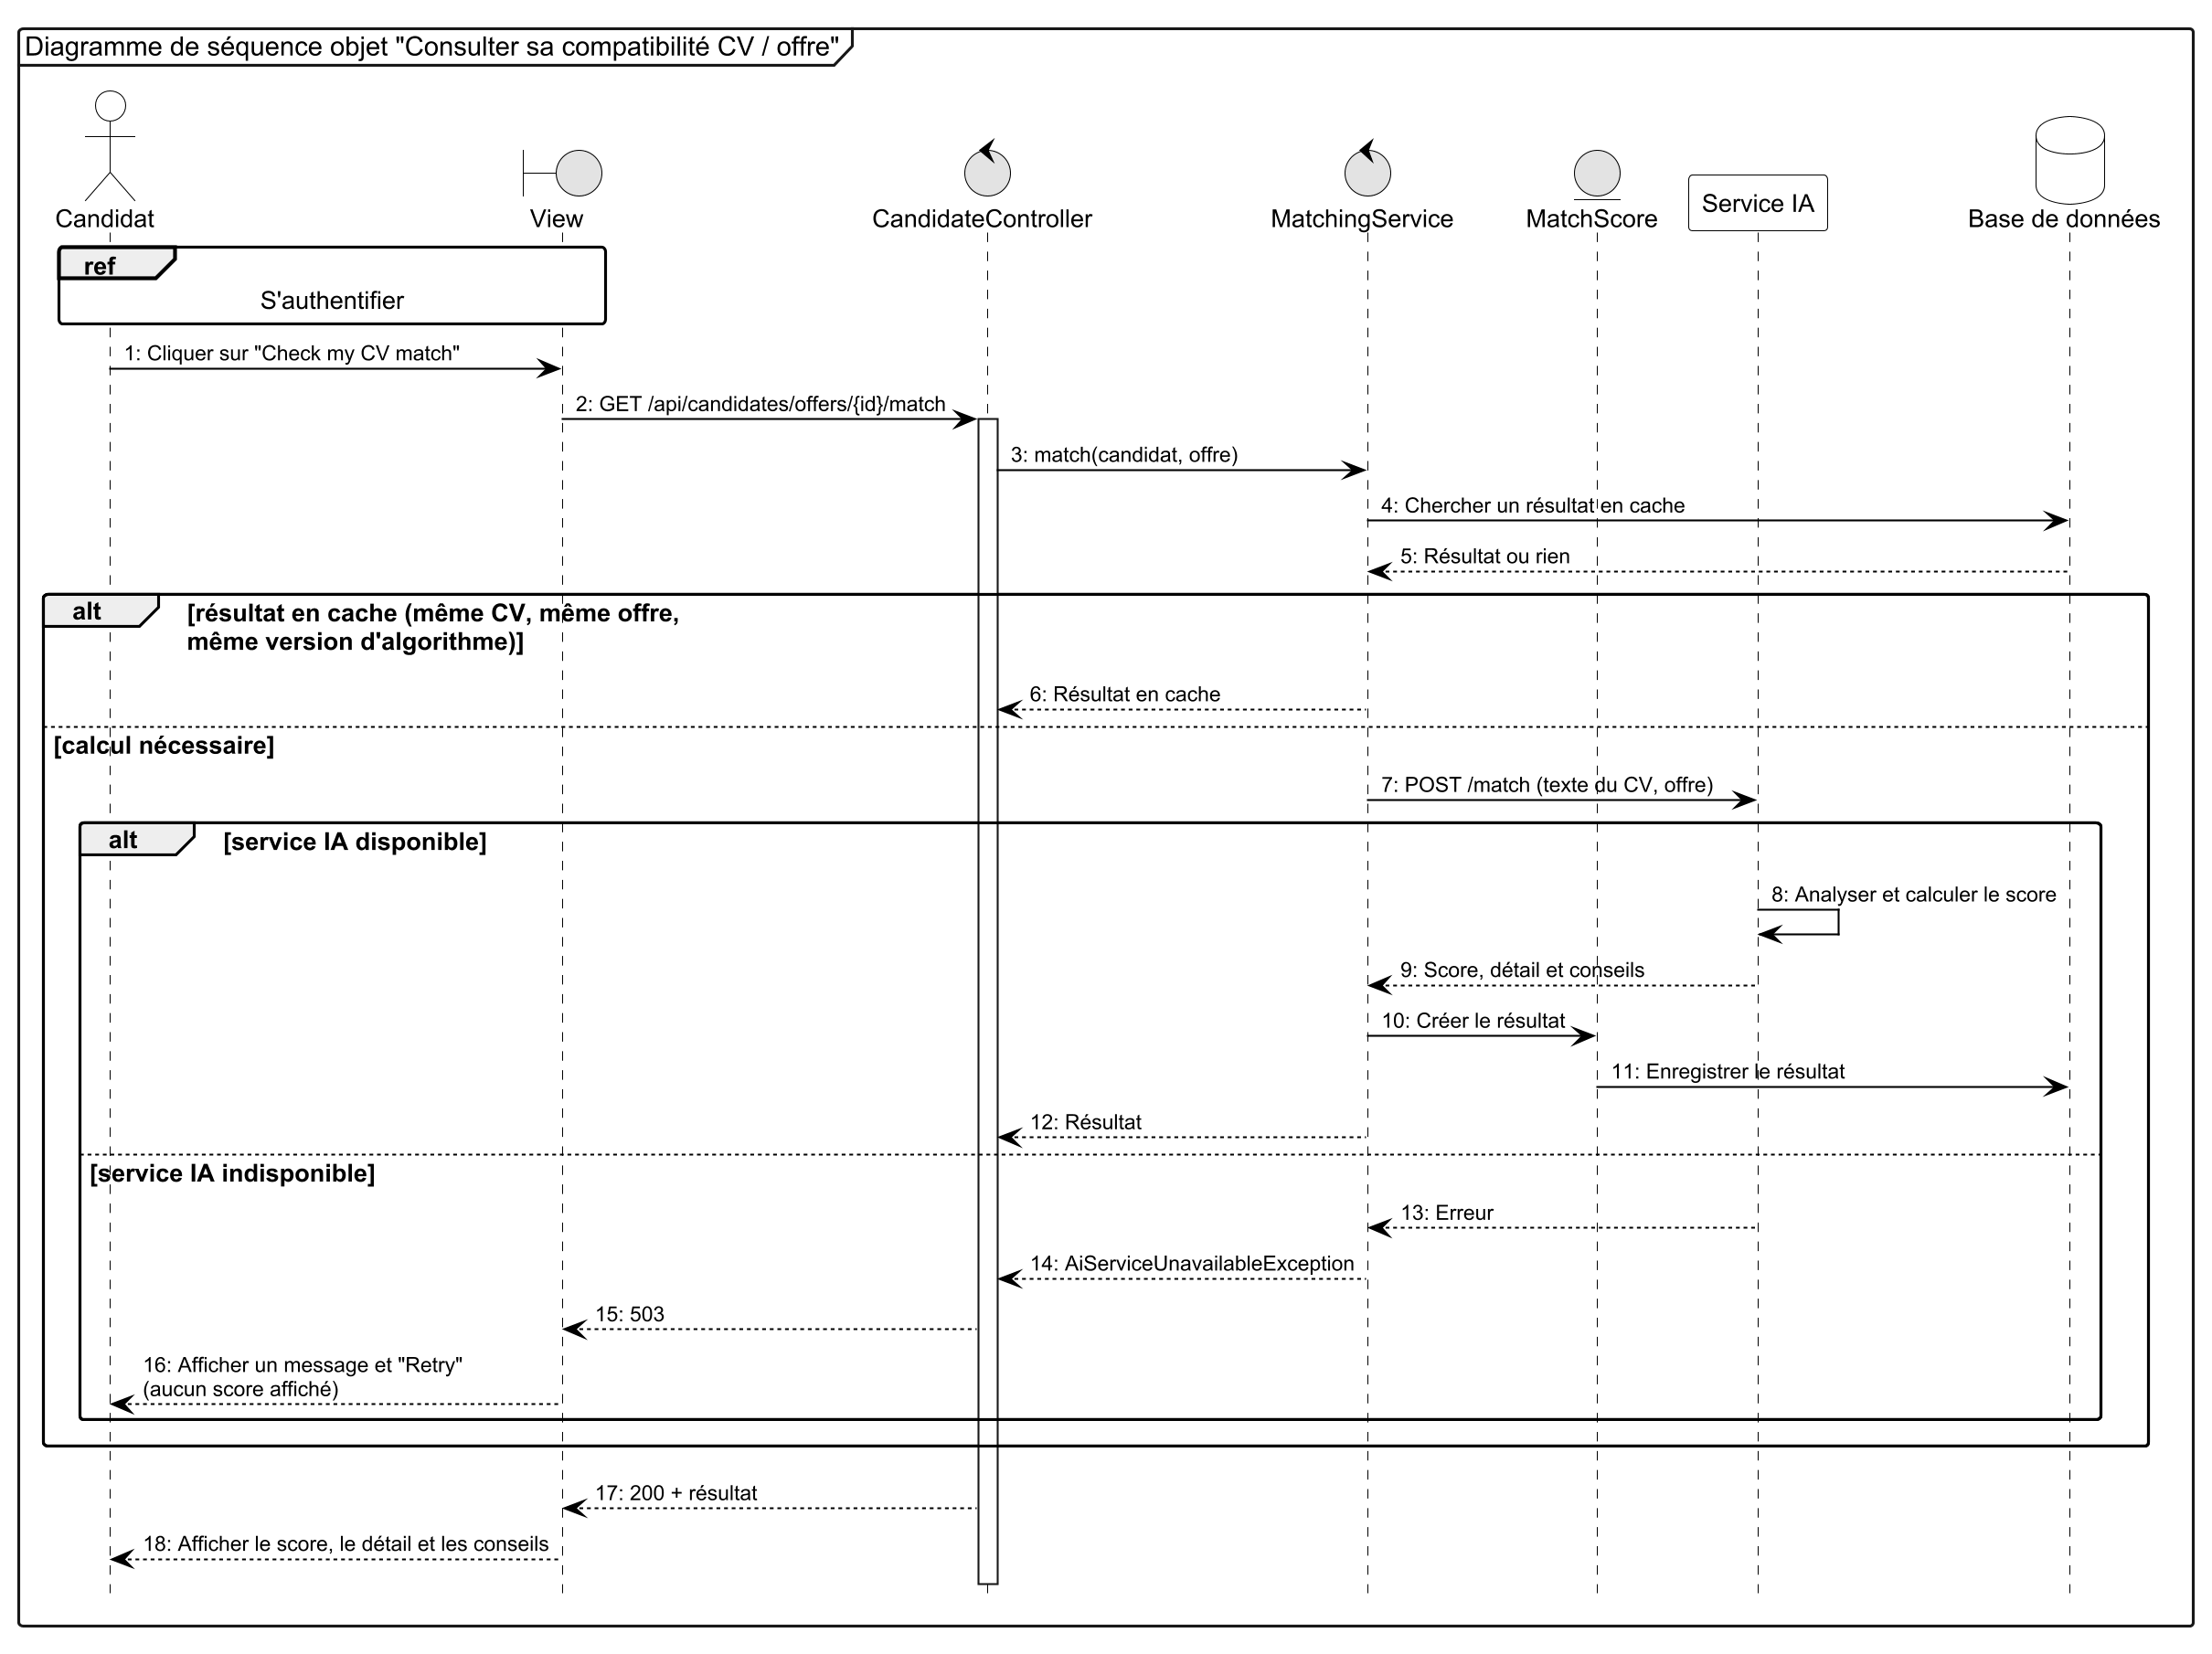
\includegraphics[width=\textwidth,height=0.72\textheight,keepaspectratio]{dso-compatibilite-cv.png}
\caption{Diagramme de séquence objet relatif au scénario « Consulter sa compatibilité CV / offre »}
\end{figure}

\section*{Conclusion}
\addcontentsline{toc}{section}{Conclusion}
Ce chapitre a présenté l'architecture de HireHub et sa conception détaillée à travers les diagrammes de classes et de séquence. Le chapitre suivant décrit la réalisation de la solution.

% ============================================================
%  CHAPITRE 4
% ============================================================
\chapter{Réalisation}
\plan

\section*{Introduction}
\addcontentsline{toc}{section}{Introduction}
Ce dernier chapitre présente l'environnement de travail, les technologies choisies, les points clés de l'implémentation, la stratégie de tests et les interfaces réalisées. Il se termine par les difficultés rencontrées.

\section{Environnement de travail}

\subsection{Environnement matériel}
% TODO Marwa: complétez avec les caractéristiques réelles de votre ordinateur.
\begin{table}[H]
\centering
\begin{tabularx}{0.8\textwidth}{|p{4.5cm}|L|}
\hline
\rowcolor{headgray}\thead{Caractéristique} & \thead{Valeur} \\ \hline
Processeur & \ldots \\ \hline
Mémoire RAM & \ldots \\ \hline
Système d'exploitation & Windows 11 Professionnel \\ \hline
\end{tabularx}
\caption{Caractéristiques du poste de travail}
\end{table}

\subsection{Environnement logiciel}
\begin{table}[H]
\centering
\begin{tabularx}{\textwidth}{|p{4cm}|L|}
\hline
\rowcolor{headgray}\thead{Outil} & \thead{Utilisation} \\ \hline
IntelliJ IDEA & Développement du backend Spring Boot \cite{intellij} \\ \hline
Visual Studio Code & Développement du frontend React et du service Python \cite{vscode} \\ \hline
Git / GitHub & Gestion de versions ; GitHub Actions pour l'intégration continue \cite{github} \\ \hline
Docker / Docker Compose & Conteneurisation des services \cite{docker} \\ \hline
MySQL Workbench & Visualisation de la base de données \\ \hline
Postman / Swagger UI & Tests manuels et documentation de l'API \cite{springdoc} \\ \hline
Mailpit & Boîte e-mail locale pour le développement et les tests \cite{mailpit} \\ \hline
PlantUML & Diagrammes UML (sources versionnées avec le code) \cite{plantuml} \\ \hline
Overleaf / LaTeX & Rédaction du rapport \\ \hline
\end{tabularx}
\caption{Environnement logiciel}
\end{table}

\section{Choix techniques}

\begin{table}[H]
\centering\small
\begin{tabularx}{\textwidth}{|p{2.7cm}|p{4.8cm}|L|}
\hline
\rowcolor{headgray}\thead{Couche} & \thead{Technologies} & \thead{Justification} \\ \hline
Frontend & React 19, Vite, React Router, Axios \cite{react} & Interface réactive à composants ; Vite rend le développement rapide. \\ \hline
Backend & Java 17, Spring Boot 3.5, Spring Security, Spring Data JPA, Flyway, Bucket4j \cite{springboot} & Cadre robuste et typé pour la sécurité, les règles métier et les données. \\ \hline
Service IA & Python 3.12, FastAPI, sentence-transformers, pypdf, python-docx, BeautifulSoup \cite{fastapi,sbert} & L'écosystème Python est le plus adapté au traitement du texte et aux modèles de langue. \\ \hline
Données & MySQL 8 & Base relationnelle fiable ; schéma versionné avec Flyway. \\ \hline
Tests & JUnit 5, MockMvc, Testcontainers, pytest, Vitest, Playwright \cite{playwright} & Tests à tous les niveaux, sur une vraie base MySQL et dans un vrai navigateur. \\ \hline
Déploiement & Docker, nginx, GitHub Actions & Environnement reproductible et vérification automatique de chaque modification. \\ \hline
\end{tabularx}
\caption{Technologies utilisées et justification}
\end{table}

Toutes les technologies utilisées sont gratuites et open source ; les vrais e-mails passent par le SMTP gratuit de Gmail avec un mot de passe d'application.

\section{Réalisation des fonctionnalités clés}

\subsection{Sécurité et session}
La session de l'utilisateur est un jeton JWT placé dans un cookie \textbf{HttpOnly} : le JavaScript de la page ne peut pas le lire, ce qui empêche son vol en cas de faille XSS. Le cookie est envoyé uniquement à l'API (\texttt{Path=/api}) et jamais lors d'une requête provenant d'un autre site (\texttt{SameSite=Strict}).

\begin{lstlisting}[language=Java,caption={Création du cookie de session (SessionCookie.java)}]
private ResponseCookie.ResponseCookieBuilder base(String value) {
    return ResponseCookie.from(NAME, value)
            .httpOnly(true).secure(secure)
            .sameSite("Strict").path(PATH);
}
\end{lstlisting}

Les requêtes qui modifient des données (POST, PUT, DELETE) et qui utilisent ce cookie doivent aussi porter un jeton CSRF dans un en-tête. Les clients qui ne sont pas des navigateurs (Swagger, scripts) envoient le jeton dans l'en-tête \texttt{Authorization}.

\begin{lstlisting}[language=Java,caption={Quand le jeton CSRF est exigé (SecurityConfig.java)}]
static boolean needsCsrfToken(HttpServletRequest request) {
    return !SAFE_METHODS.contains(request.getMethod())
            && request.getHeader(HttpHeaders.AUTHORIZATION) == null
            && SessionCookie.read(request).isPresent();
}
\end{lstlisting}

Les autorisations sont vérifiées dans les services : un recruteur ne peut traiter que les candidatures de ses propres offres. Une action interdite renvoie le code \textbf{403} (\texttt{ForbiddenException}), et une donnée invalide le code 400.

\begin{lstlisting}[language=Java,caption={Contrôle du propriétaire et de l'état (ApplicationService.java)}]
if (currentUser.getRole() != Role.RECRUITER || !isOwnerRecruiter(existingApp, currentUser)) {
    throw new ForbiddenException("You are not allowed to update this application.");
}
if (existingApp.getStatus() != ApplicationStatus.PENDING) {
    throw new BadRequestException("Application has already been processed.");
}
\end{lstlisting}

Enfin, la connexion et la réinitialisation du mot de passe sont protégées contre les attaques par force brute (Bucket4j) : par exemple, cinq échecs de connexion par adresse e-mail en quinze minutes, et dix demandes de réinitialisation par adresse IP en quinze minutes. Au-delà, l'API répond 429 avec un en-tête \texttt{Retry-After}.

\subsection{Analyse et compatibilité du CV}
Lors du dépôt, le texte du CV (PDF ou DOCX) est extrait par le service IA. Pour comparer un CV à une offre, le service analyse l'offre (compétences requises et souhaitées, années d'expérience, diplôme, langues) et le CV, puis calcule un score par catégorie (tableau \ref{tab:poids}).

\begin{table}[H]
\centering
\begin{tabularx}{\textwidth}{|p{3cm}|p{1.6cm}|L|}
\hline
\rowcolor{headgray}\thead{Catégorie} & \thead{Poids} & \thead{Mesure} \\ \hline
Compétences & 45 \% & Compétences requises et souhaitées, avec synonymes (« JS » = JavaScript, Spring Boot implique Spring). \\ \hline
Expérience & 20 \% & Années dans des postes utilisant les compétences de l'offre. \\ \hline
Pertinence & 15 \% & Similarité sémantique multilingue entre le CV et l'offre (français et anglais). \\ \hline
Formation & 10 \% & Niveau de diplôme. \\ \hline
Langues & 10 \% & Langues et niveaux demandés. \\ \hline
\end{tabularx}
\caption{Pondération du score de compatibilité}
\label{tab:poids}
\end{table}

Si l'offre ne mentionne pas une catégorie, celle-ci est ignorée et les autres poids sont recalculés : le candidat n'est jamais pénalisé pour un critère absent.

\begin{lstlisting}[language=Python,caption={Calcul du score global (scoring.py)}]
WEIGHTS = {"skills": 0.45, "experience": 0.20, "education": 0.10,
           "languages": 0.10, "relevance": 0.15}

active_weight = sum(WEIGHTS[name] for name, cat in categories.items() if cat["applicable"])
for name, cat in categories.items():
    cat["effective_weight"] = round(WEIGHTS[name] / active_weight, 3) if cat["applicable"] else 0.0
overall = round(sum(cat["score"] * cat["effective_weight"]
                    for cat in categories.values() if cat["applicable"]))
\end{lstlisting}

La similarité sémantique utilise le modèle multilingue \texttt{paraphrase-multilingual-\allowbreak MiniLM-L12-v2} \cite{sbert}, qui fonctionne sur un simple processeur et permet de comparer un CV français à une offre anglaise. Le résultat est mis en cache selon l'empreinte SHA-256 du CV, le texte de l'offre et la version de l'algorithme : il n'est recalculé que si l'un d'eux change.

\subsection{Import du profil entreprise}
À l'inscription, le recruteur peut indiquer le site web de son entreprise. Le service IA lit les pages publiques (données schema.org, balises meta, sections « Mission », « Vision », « Valeurs ») et remplit uniquement les champs encore vides ; ces champs sont marqués « From your website » jusqu'à ce que le recruteur les vérifie. Pour éviter les attaques \textbf{SSRF}, le service refuse les adresses internes ou privées.

\subsection{Rédaction assistée}
Les boutons « Draft my bio » et « Draft a description » proposent un texte construit \textbf{uniquement} à partir des données saisies par l'utilisateur. Un modèle de langue local (Ollama) peut être activé en option pour reformuler le texte ; des garde-fous vérifient alors qu'il n'ajoute aucune information inventée.
% TODO Marwa: précisez le modèle Ollama utilisé si vous l'avez testé.

\subsection{E-mails}
Deux e-mails sont envoyés, en HTML et en texte brut, avec l'identité visuelle de HireHub : l'e-mail de bienvenue et le lien de réinitialisation du mot de passe. L'envoi est \textbf{asynchrone} et se fait après l'enregistrement en base : si le serveur SMTP échoue, l'action de l'utilisateur réussit quand même et l'erreur est journalisée. Le mode d'envoi se choisit par configuration : Mailpit en développement et pour les tests, Gmail SMTP pour les vrais e-mails.

\subsection{Base de données et exploitation}
\begin{itemize}
  \item \textbf{Flyway} : le schéma est décrit par des scripts SQL versionnés ; Hibernate vérifie seulement que les entités correspondent au schéma (\texttt{ddl-auto=validate}).
  \item \textbf{Profils} : configuration séparée pour le développement, les tests et la production.
  \item \textbf{Swagger UI} (springdoc) documente l'API ; \textbf{Actuator} expose l'état de santé du backend et du service IA.
  \item \textbf{Journaux} : chaque requête reçoit un identifiant (\texttt{X-Request-Id}) transmis au service IA et renvoyé dans les messages d'erreur ; en production, les journaux sont structurés (format JSON).
\end{itemize}

\subsection{Conteneurisation avec Docker}
La conteneurisation a été mise en place pour rendre l'installation reproductible :
\begin{itemize}
  \item un \texttt{Dockerfile} par service : le backend (build Maven puis image Java), le frontend (build Vite puis serveur nginx qui redirige \texttt{/api} vers le backend) et le service IA (le modèle de langue est téléchargé lors de la construction de l'image) ;
  \item un fichier \texttt{docker-compose.yml} qui lance MySQL, le backend, le service IA, le frontend et Mailpit, avec des contrôles de santé (\emph{healthchecks}) et des volumes pour la base de données et les fichiers déposés ;
  \item le service IA et MySQL restent sur le réseau interne de Docker : seul nginx est accessible depuis l'extérieur.
\end{itemize}
L'exécution complète de la suite de tests Playwright sur la pile Docker est en cours de finalisation et constitue la prochaine étape du projet.

\subsection{Intégration continue}
Un workflow GitHub Actions vérifie chaque modification : tests du backend (\texttt{mvn verify}, avec une base MySQL lancée automatiquement par Testcontainers), tests du service IA (pytest), analyse statique et tests du frontend (ESLint, Vitest) et construction de l'application.

\section{Tests}
Les tests ont été automatisés à tous les niveaux (tableau \ref{tab:tests}). Les tests de bout en bout lancent toute l'application et jouent des parcours réels dans un navigateur, par exemple : inscription puis arrivée connectée sur le tableau de bord, réception de l'e-mail de réinitialisation dans Mailpit et changement du mot de passe, ou session expirée.

\begin{table}[H]
\centering\small
\begin{tabularx}{\textwidth}{|p{3cm}|p{3.4cm}|L|p{1.4cm}|}
\hline
\rowcolor{headgray}\thead{Niveau} & \thead{Outils} & \thead{Ce qui est testé} & \thead{Tests} \\ \hline
Backend & JUnit 5, MockMvc, Testcontainers & Services, sécurité (cookie, CSRF, 403), limites de débit, e-mails, migrations & 329 \\ \hline
Service IA & pytest & Extraction du texte, analyse des CV français et anglais, score, import d'entreprise, rédaction & 122 \\ \hline
Frontend & Vitest & Composants, formulaires, validation des profils & 74 \\ \hline
Bout en bout & Playwright & Parcours complets candidat et recruteur, e-mails, navigation & 24 \\ \hline
\end{tabularx}
\caption{Tests automatisés (dernière exécution complète)}
\label{tab:tests}
\end{table}
% TODO Marwa: mettez à jour ces nombres si vous relancez les tests avant la remise.

\section{Description des interfaces}
Les captures suivantes ont été réalisées automatiquement avec Playwright à partir des données de démonstration.

\paragraph{Interface d'authentification} Les figures suivantes montrent la page de connexion et la création de compte, où le recruteur indique aussi son entreprise et son site web.
\capture[0.9\textwidth]{02-login.jpg}{Interface d'authentification}
\capture[0.9\textwidth]{03-signup.jpg}{Interface de création de compte}

\paragraph{Vue d'ensemble du recruteur} Elle résume les offres ouvertes, les candidatures reçues et les candidatures récentes, avec les actions rapides « Accepter » et « Refuser ».
\capture{10-recruiter-overview.jpg}{Vue d'ensemble du recruteur}

\paragraph{Gestion des offres} Le recruteur consulte ses offres, en publie une nouvelle ou clôture une offre.
\capture{11-recruiter-offers.jpg}{Liste des offres du recruteur}
\capture{12-recruiter-new-offer.jpg}{Formulaire de publication d'une offre}

\paragraph{Candidatures et évaluation} Le recruteur consulte les candidatures reçues, puis évalue un candidat et planifie l'entretien.
\capture{13-recruiter-applications.jpg}{Candidatures reçues}
\capture{14-recruiter-evaluation.jpg}{Évaluation d'un candidat}

\paragraph{Statistiques et profil entreprise}
\capture{15-recruiter-statistics.jpg}{Statistiques du recruteur}
\capture{16-recruiter-company-profile.jpg}{Profil entreprise importé depuis le site web}

\paragraph{Espace candidat} Le candidat recherche des offres et consulte sa compatibilité : le score, son détail par catégorie et les conseils.
\capture{20-candidate-overview.jpg}{Vue d'ensemble du candidat}
\capture{21-candidate-offers.jpg}{Recherche d'offres}
\capture{22-candidate-cv-match.jpg}{Compatibilité du CV avec une offre}
\capture{23-candidate-applications.jpg}{Suivi des candidatures}
\capture{24-candidate-profile.jpg}{Profil du candidat avec indicateur de complétude}

\paragraph{Version mobile} L'interface s'adapte aux petits écrans : la barre de navigation reste fixe et seul le contenu défile.
\begin{figure}[H]\centering
\begin{subfigure}{0.3\textwidth}\centering
  \phoneshot{30-phone-candidate-overview.jpg}
  \caption{Vue d'ensemble}\end{subfigure}\hfill
\begin{subfigure}{0.3\textwidth}\centering
  \phoneshot{31-phone-candidate-offers.jpg}
  \caption{Offres}\end{subfigure}\hfill
\begin{subfigure}{0.3\textwidth}\centering
  \phoneshot{33-phone-recruiter-statistics.jpg}
  \caption{Statistiques}\end{subfigure}
\caption{Interfaces sur téléphone (390 px)}
\end{figure}

\section{Difficultés rencontrées et solutions}
\begin{itemize}
  \item \textbf{Limite d'envoi de fichiers} : Spring limitait les fichiers à 1 Mo et l'erreur était masquée, si bien que l'utilisateur ne savait pas pourquoi son CV était refusé. Solution : limite portée à 10 Mo et message d'erreur clair.
  \item \textbf{Communication entre le backend et le service IA} : le client HTTP de Java tentait une connexion HTTP/2 que le serveur Python (uvicorn) ne gérait pas. Solution : forcer HTTP/1.1 dans un client partagé.
  \item \textbf{Scores fictifs} : une première version affichait un score estimé quand l'analyse échouait. Ce comportement trompait l'utilisateur ; il a été supprimé : sans analyse, aucun score n'est affiché.
  \item \textbf{CV en français} : l'analyse reconnaissait mal les rubriques et les dates des CV français. Solution : rubriques et formats de dates bilingues, et un modèle de similarité multilingue.
  \item \textbf{Sécurité de la session} : le passage d'un jeton stocké dans le navigateur à un cookie HttpOnly a nécessité une protection CSRF adaptée à une application monopage.
  \item \textbf{Évolution du schéma} : la mise en place de Flyway sur une base existante a demandé un script de référence reprenant exactement le schéma en place.
\end{itemize}

\section*{Conclusion}
\addcontentsline{toc}{section}{Conclusion}
Ce chapitre a présenté l'environnement de travail, les choix techniques, la réalisation des fonctionnalités clés, les tests et les interfaces de HireHub, ainsi que les difficultés rencontrées et leurs solutions.

% ============================================================
%  CONCLUSION GÉNÉRALE
% ============================================================
\chapter*{Conclusion générale et perspectives}
\addcontentsline{toc}{chapter}{Conclusion générale et perspectives}
\markboth{Conclusion générale et perspectives}{}

Ce stage d'été chez Proxym-IT a été une expérience professionnelle enrichissante. Le développement de la plateforme HireHub m'a permis de travailler sur toute la chaîne de réalisation d'une application web : analyse des besoins, modélisation UML, conception d'une architecture à plusieurs services, développement d'une API REST sécurisée, d'un service d'analyse de CV en Python et d'une interface React, puis tests automatisés, intégration continue et conteneurisation.

La version actuelle couvre l'ensemble des besoins identifiés : gestion des offres et des candidatures, compatibilité CV / offre explicable, évaluation des candidats, statistiques, import du profil entreprise et e-mails réels. Sur le plan technique, ce projet m'a permis d'approfondir la sécurité des applications web, le traitement automatique du texte et les bonnes pratiques de qualité logicielle. Sur le plan personnel, il m'a appris à être autonome, rigoureuse et à structurer un projet de bout en bout.

Plusieurs évolutions sont envisagées :

\paragraph{Finalisation du déploiement} Terminer la validation de la pile Docker avec la suite de tests de bout en bout, puis déployer l'application sur un serveur accessible en HTTPS, afin que les liens envoyés par e-mail fonctionnent depuis n'importe quel réseau.

\paragraph{Assistant « Interroger mes candidats » (RAG)} Permettre au recruteur de poser des questions en langage naturel sur ses candidats (« Qui a de l'expérience en Spring Boot et parle anglais ? »). Les CV seraient découpés en passages et indexés sous forme de vecteurs ; pour chaque question, seuls les passages pertinents seraient retrouvés et fournis à un modèle de langue, qui répondrait en citant ses sources. La recherche serait filtrée par la liste des candidats autorisés pour ce recruteur, pour qu'il ne voie jamais d'autres données. Des règles d'équité interdiraient les critères discriminatoires (âge, sexe, origine), et la qualité serait mesurée par le rappel des passages retrouvés (\emph{recall@k}) et la fidélité des réponses aux sources (\emph{faithfulness}). La figure \ref{fig:rag} résume l'architecture envisagée.

\begin{figure}[H]\centering
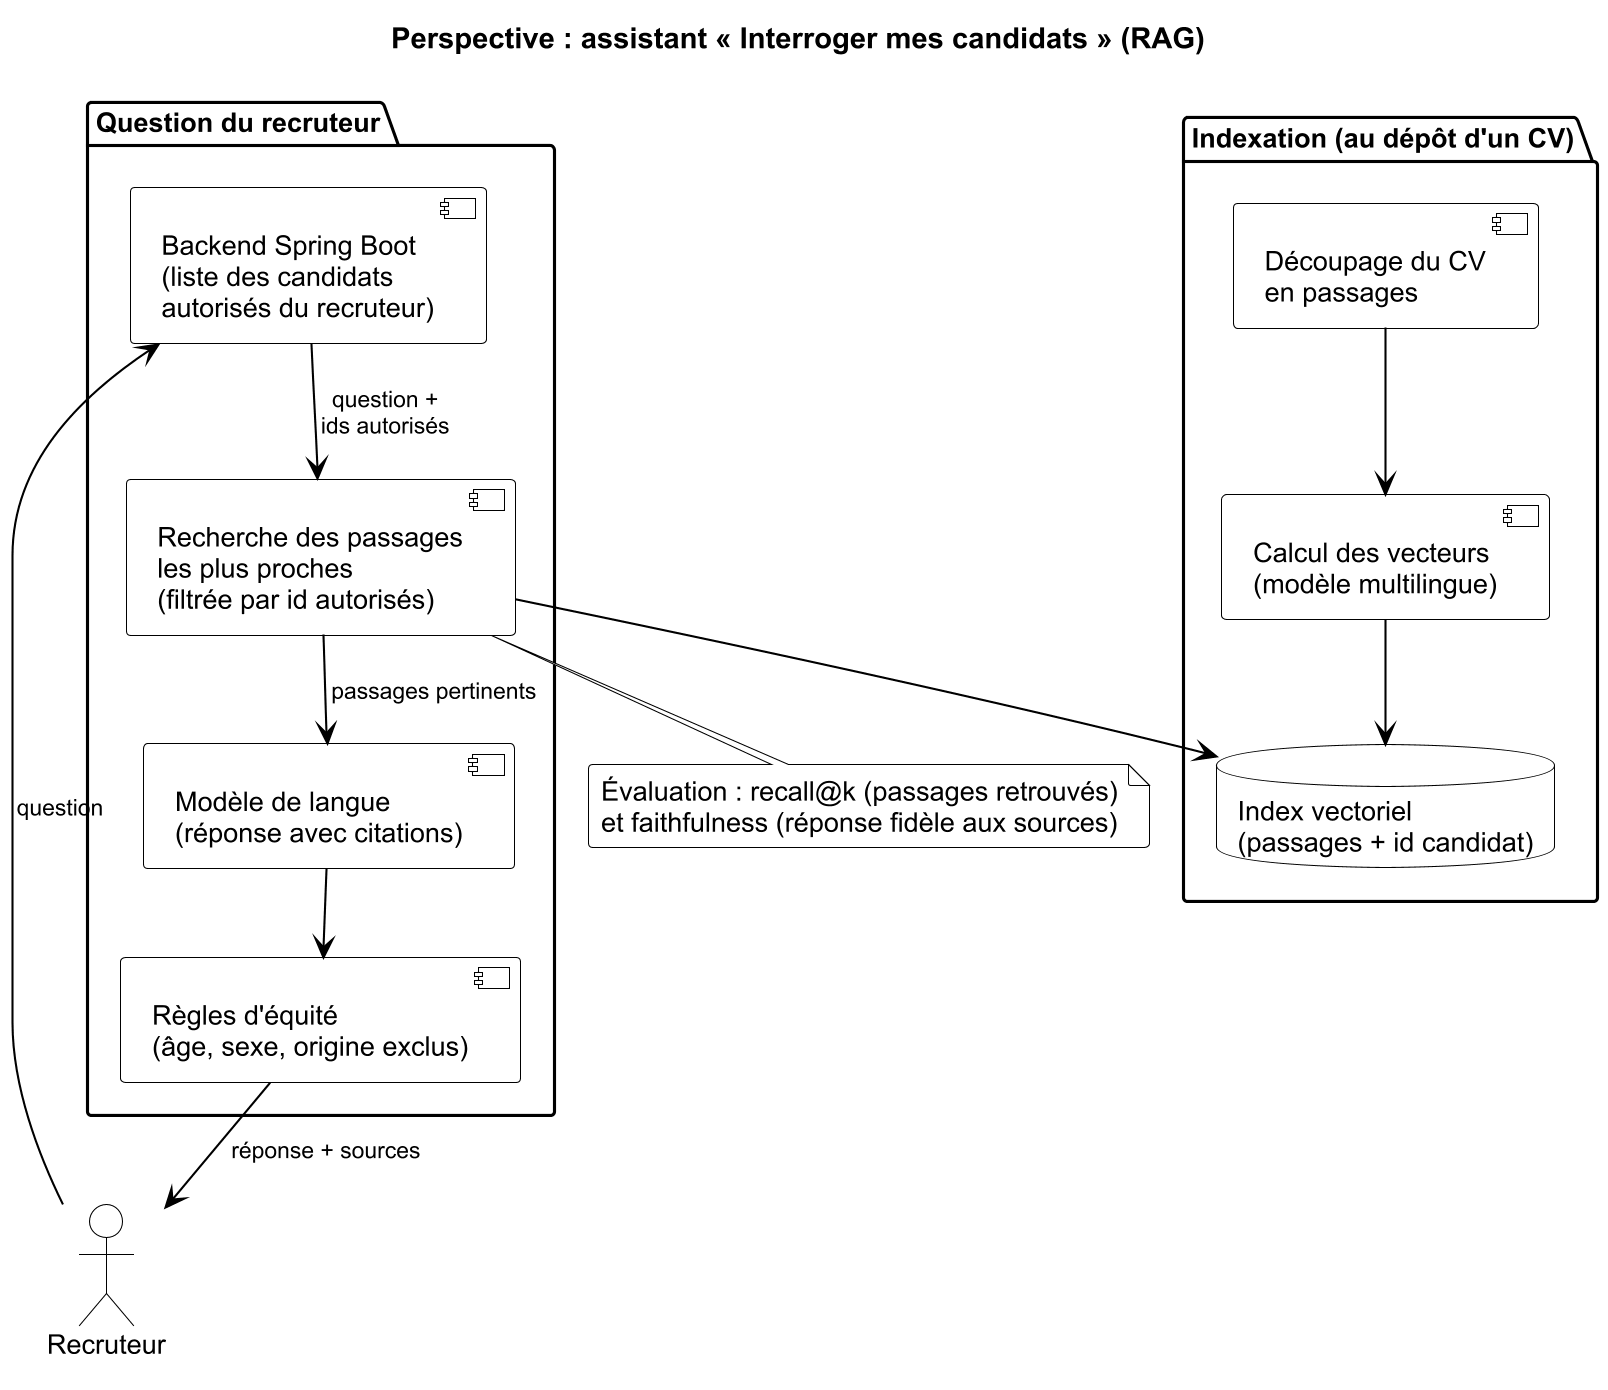
\includegraphics[width=0.9\textwidth,height=0.6\textheight,keepaspectratio]{perspective-rag.png}
\caption{Architecture envisagée de l'assistant RAG « Interroger mes candidats »}
\label{fig:rag}
\end{figure}

\paragraph{Questions d'entretien personnalisées} Générer, à partir de l'offre et du CV, des questions ciblant les compétences à vérifier et les écarts détectés par l'analyse.

\paragraph{Assistant pour le candidat} Aider le candidat à améliorer son CV pour une offre donnée, à partir des conseils déjà produits par l'analyse de compatibilité.

Ces perspectives confirment le potentiel de HireHub à évoluer vers un outil de recrutement plus intelligent, tout en restant transparent et respectueux des données des utilisateurs.

% ============================================================
%  NETOGRAPHIE
% ============================================================
% TODO Marwa: ajustez les dates de consultation si besoin.
\chapter*{Netographie}
\addcontentsline{toc}{chapter}{Netographie}
\markboth{Netographie}{}
\renewcommand{\bibname}{}
\begingroup
\renewcommand{\chapter}[2]{}
\begin{thebibliography}{99}
\bibitem{proxym} Proxym-IT, \url{https://www.proxym-group.com/}, (consulté le 05/10/2026).
\bibitem{springboot} Spring Boot, \url{https://docs.spring.io/spring-boot/}, (consulté le 05/10/2026).
\bibitem{springsecurity} Spring Security, \url{https://docs.spring.io/spring-security/}, (consulté le 05/10/2026).
\bibitem{react} React, \url{https://react.dev/}, (consulté le 05/10/2026).
\bibitem{fastapi} FastAPI, \url{https://fastapi.tiangolo.com/}, (consulté le 05/10/2026).
\bibitem{sbert} Sentence-Transformers, \url{https://www.sbert.net/}, (consulté le 05/10/2026).
\bibitem{playwright} Playwright, \url{https://playwright.dev/}, (consulté le 05/10/2026).
\bibitem{docker} Docker, \url{https://docs.docker.com/}, (consulté le 05/10/2026).
\bibitem{springdoc} springdoc-openapi, \url{https://springdoc.org/}, (consulté le 05/10/2026).
\bibitem{mailpit} Mailpit, \url{https://mailpit.axllent.org/}, (consulté le 05/10/2026).
\bibitem{plantuml} PlantUML, \url{https://plantuml.com/fr/}, (consulté le 05/10/2026).
\bibitem{intellij} IntelliJ IDEA, \url{https://www.jetbrains.com/idea/}, (consulté le 05/10/2026).
\bibitem{vscode} Visual Studio Code, \url{https://code.visualstudio.com/}, (consulté le 05/10/2026).
\bibitem{github} GitHub Actions, \url{https://docs.github.com/actions}, (consulté le 05/10/2026).
\bibitem{owasp} OWASP, Cross-Site Request Forgery Prevention Cheat Sheet, \url{https://cheatsheetseries.owasp.org/}, (consulté le 05/10/2026).
\end{thebibliography}
\endgroup

% ============================================================
%  RÉSUMÉ / ABSTRACT (dernière page, comme dans les modèles)
% ============================================================
\clearpage
\thispagestyle{empty}
\section*{Résumé}
Ce rapport présente le travail réalisé lors de mon stage d'été au sein de Proxym-IT : la conception et le développement de \textbf{« HireHub : plateforme de gestion des offres d'emploi et des candidatures »}. L'application permet aux recruteurs de publier leurs offres, de traiter et d'évaluer les candidatures, et aux candidats de rechercher des offres et de postuler. Un service d'analyse calcule un score de compatibilité explicable entre le CV et l'offre, et importe le profil d'une entreprise depuis son site web. La solution repose sur React, Spring Boot, FastAPI et MySQL ; elle est sécurisée, testée automatiquement et conteneurisée avec Docker.

\noindent\textbf{Mots clés :} Recrutement, Analyse de CV, Spring Boot, React, FastAPI, Docker.

\vspace{1.5cm}
\section*{Abstract}
This report presents the work carried out during my summer internship at Proxym-IT: the design and development of \textbf{“HireHub: a job offer and application management platform”}. Recruiters publish offers, review and evaluate applications, while candidates search for offers and apply. An analysis service computes an explainable match score between a CV and an offer, and imports a company profile from its website. The solution is built with React, Spring Boot, FastAPI and MySQL; it is secured, covered by automated tests and containerised with Docker.

\noindent\textbf{Keywords:} Recruitment, CV analysis, Spring Boot, React, FastAPI, Docker.

\end{document}
